\documentclass{article}
\usepackage[utf8]{inputenc}
\usepackage{tabularx} % extra features for tabular environment
\usepackage{amsmath}  % improve math presentation
\usepackage{graphicx} % takes care of graphic including machinery
\usepackage{listings}
\usepackage{xcolor}

\definecolor{codegreen}{rgb}{0,0.6,0}
\definecolor{codegray}{rgb}{0.5,0.5,0.5}
\definecolor{codepurple}{rgb}{0.58,0,0.82}
\definecolor{backcolour}{rgb}{1, 1, 1}

\lstdefinestyle{mystyle}{
    backgroundcolor=\color{backcolour},   
    commentstyle=\color{codegreen},
    keywordstyle=\color{magenta},
    numberstyle=\tiny\color{codegray},
    stringstyle=\color{codepurple},
    basicstyle=\ttfamily\footnotesize,
    breakatwhitespace=false,         
    breaklines=true,                 
    captionpos=b,                    
    keepspaces=true,                      
    showspaces=false,                
    showstringspaces=false,
    showtabs=false,                  
    tabsize=2
}

\lstset{style=mystyle}

\usepackage{xspace}
\usepackage{multirow}
\usepackage{tikz}
\usepackage{enumitem}
\usetikzlibrary{babel}
\usepackage[american]{circuitikz}
\usetikzlibrary{calc}
\usepackage{siunitx}
\usepackage{pgfplots}
\usepackage[skins,theorems]{tcolorbox}
\tcbset{highlight math style={enhanced,
  colframe=red,colback=white,arc=0pt,boxrule=1pt}}
\pgfplotsset{width=10cm,compat=1.9}
\usepackage[margin=1in,letterpaper]{geometry} % decreases margins
\usepackage{cite} % takes care of citations
\usepackage[final]{hyperref} % adds hyper links inside the generated PDF file
\hypersetup{
colorlinks=true,       % false: boxed links; true: colored links
linkcolor=blue,        % color of internal links
citecolor=blue,        % color of links to bibliography
filecolor=magenta,     % color of file links
urlcolor=blue        
}
\begin{document}

\title{\textbf{Homework Assignment 1}}
\author{\textbf{TADIPATRI UDAY KIRAN REDDY}\\\textbf{EE19BTECH11038}}
\maketitle

\section{SPICE Analyses}
\subsection*{(a)}
\textbf{SPICE Netlist}
\begin{lstlisting}
Vin N001 0 2.5
R1 Out N001 1k
C1 Out N002 1u
R2 N002 0 100
.op
.backanno
.end
\end{lstlisting}
\textbf{TestBench}\\
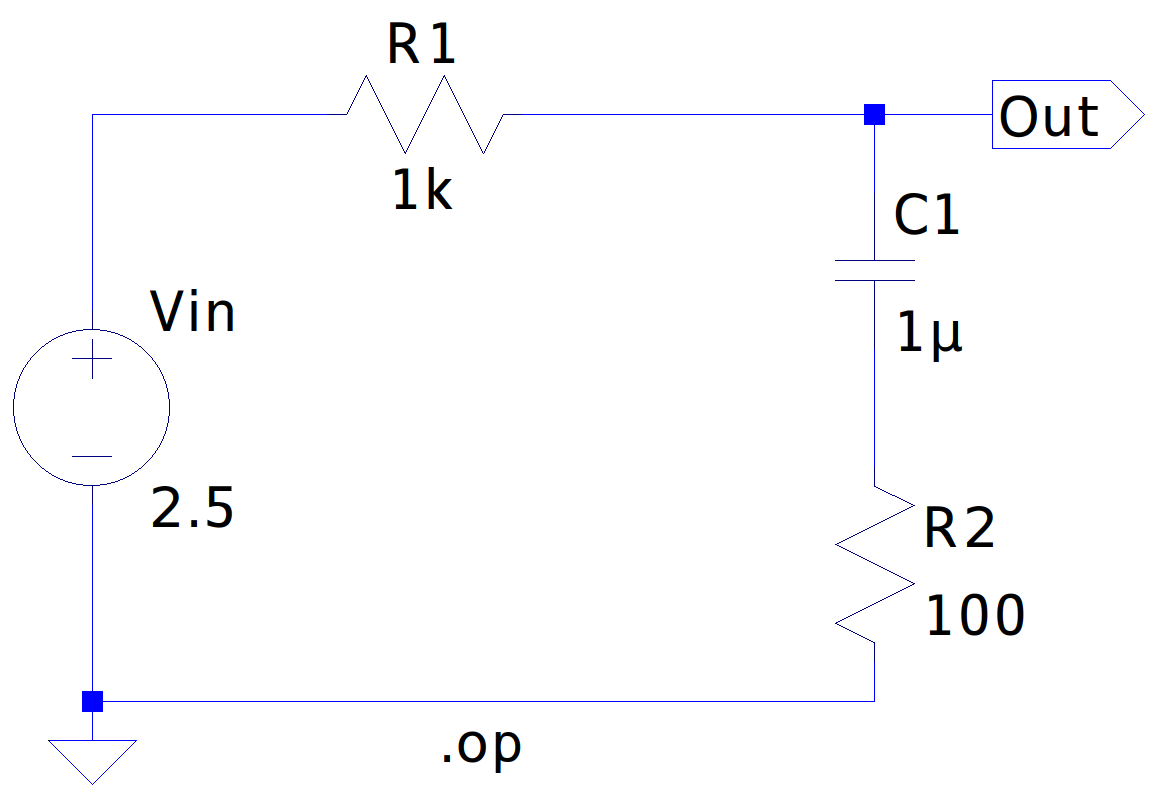
\includegraphics[scale=0.2]{./figs/Q1_a_tb.png}\\
\textbf{Operating point simulation results}\\
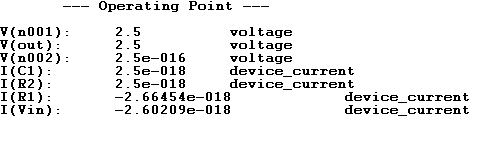
\includegraphics[scale=0.7]{./figs/Q1_a_op.png}\\
\textbf{Operating point at $V_{out}$ is 2.5V}.

\subsection*{(b)}
Applying KVL in the given circuit we get,
\begin{equation*}
V_{in} = 1k{\si{\ohm}}xi + \frac{\int_0^t{i dt}}{1\mu} + 100xi
\end{equation*}
In Laplacian domain we get,
\begin{gather*}
V_{in}(s) = \left(1100 + \frac{10^6}{s}\right)I(s)\\
\implies \frac{V_{out}(s)}{V_{in}(s)} = \frac{\left(100 + \frac{10^6}{s}\right)I(s)}{\left(1100 + \frac{10^6}{s}\right)I(s)}\\
\tcbhighmath[drop fuzzy shadow]{\frac{V_{out}(s)}{V_{in}(s)} = \frac{s + 10000}{11s + 10000}}
\end{gather*}
At f = 100Hz,\\
\begin{equation*}
\frac{V_{out}(s)}{V_{in}(s)} = 0.82426\angle{-31.055^o}
\end{equation*}
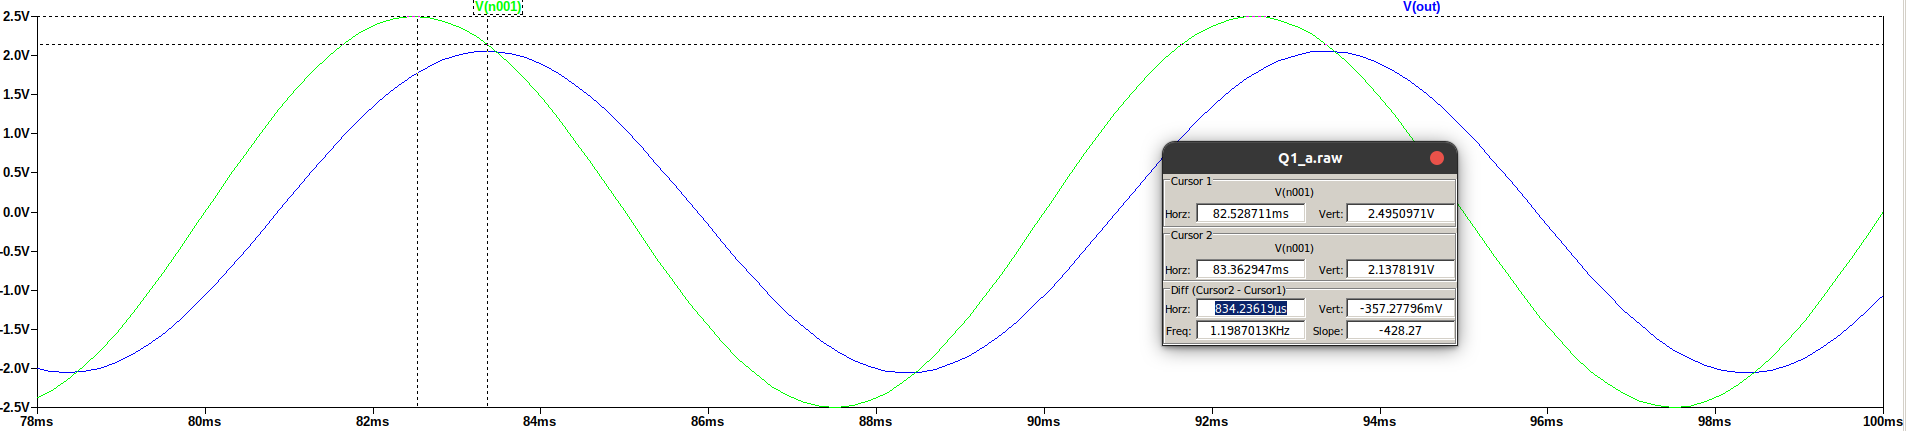
\includegraphics[scale=0.28]{./figs/Q1_b_ts.png}\\
Observe that difference between peaks is 834$\mu$s, and time period is 10ms(or 10000$\mu$s), where $V_{out}$ is lagging.
\begin{equation*}
\Delta \phi = -360\frac{834 \mu s}{10000 \mu s} \implies \Delta \phi = -30.024^o
\end{equation*}
At f = 1MHz,\\
\begin{equation*}
\frac{V_{out}(s)}{V_{in}(s)} = 0.0909\angle{-0.0829^o}
\end{equation*}
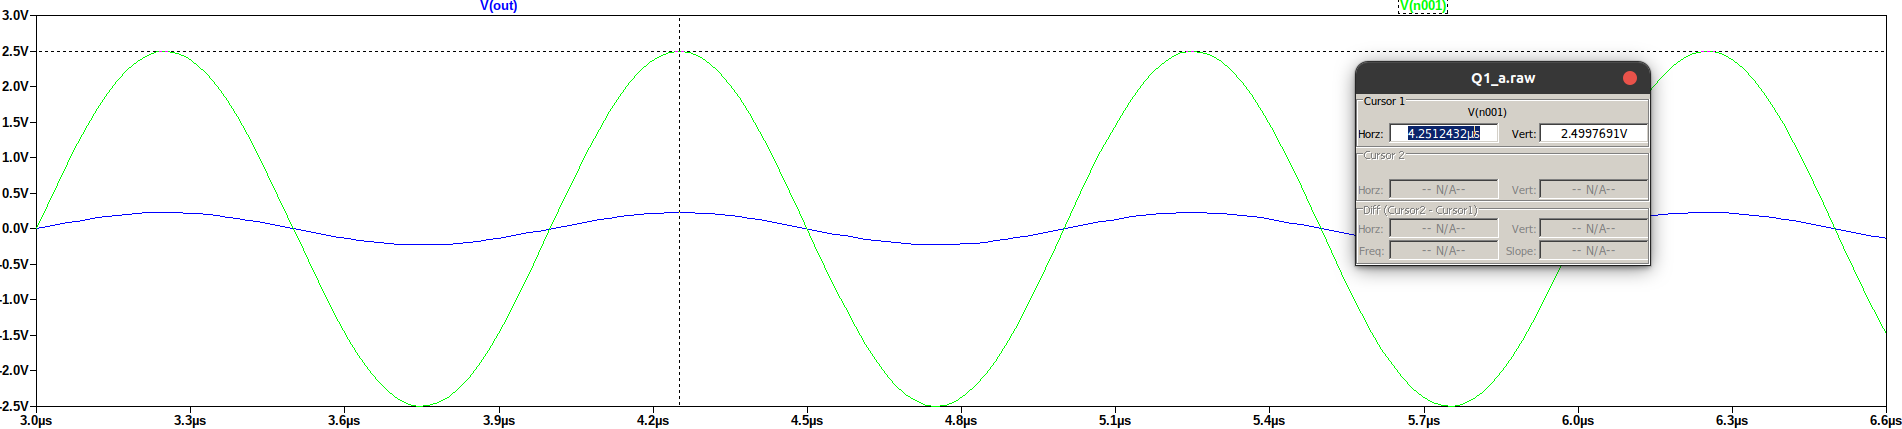
\includegraphics[scale=0.28]{./figs/Q1_b_tr_1.png}\\
Observe that difference between peaks is approximatly 0.\\
Finally,\\
\begin{center}
\begin{tabular}{|c|c|c|}
\hline
f & $\Delta {\phi}_{analytical}$ & $\Delta {\phi}_{simulated}$ \\
\hline
100Hz & -31.05$5^o$ & -30.2$4^o$  \\
\hline
1MHz & -0.082$9^o$ & $0^o$\\
\hline
\end{tabular}
\end{center}

\subsection*{(c)}
\textbf{Bode Plot}\\
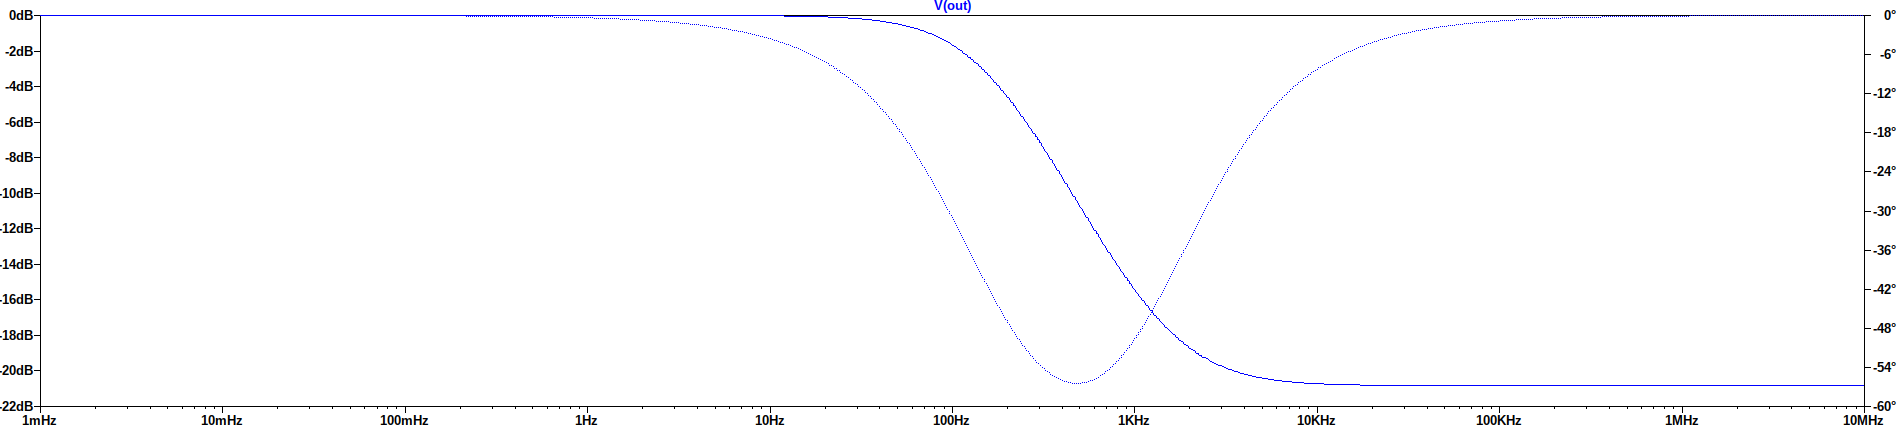
\includegraphics[scale=0.28]{./figs/Q1_c.png}\\
 \newline
\textbf{3-db Point}\\
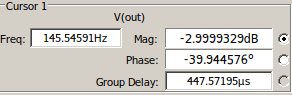
\includegraphics[scale=0.5]{./figs/Q1_c_1.png}\\
 \newline
From above obstained transfer function we get,\\
\begin{gather*}
-3 = 20log_{10}\left(\left|\frac{s + 10000}{11s + 10000}\right|\right)\\
\implies \left|\frac{j{\omega} + 10000}{11j{\omega} + 10000}\right| ^2 = \frac{1}{2}\\
\left(\frac{{\omega}^2 + 10^8}{121{\omega}^2 + 10^8}\right)= \frac{1}{2}
\implies \omega = 916.7 rad s^{-1}\\
\implies \tcbhighmath[drop fuzzy shadow]{f_{3-db} = 145.89 Hz} 
\end{gather*}
Corresponding phase lag would be,\\
\begin{gather*}
\Delta {\phi}_{3-db} = tan^{-1} \left(\frac{10000}{2{\pi}f}\right) - tan^{-1} \left(\frac{10000}{22{\pi}f}\right)\\
\implies \tcbhighmath[drop fuzzy shadow]{\Delta {\phi}_{3-db} = -39.99^o}
\end{gather*}

\section{Analytic calculations vs SPICE simulations}
\subsection*{(a)}
Applying KVL,\\
\begin{gather*}
2.5 = 2k{\si{\ohm}}*I_D + V_D + 2k{\si{\ohm}}*I_D + V_D\\
\implies I_D = \frac{2.5 - 2V_D}{4000}\\
\tcbhighmath[drop fuzzy shadow]{I_D = 275{\mu}A}
\end{gather*}
\subsection*{(b)}
Current through diode is characterized by,
\begin{equation*}
i_D = I_s\left(e^{\frac{V_D}{V_T}} - 1\right)
\end{equation*}
Where $I_s$ is Saturation current which is $10^{-14}$A and $V_T$ is thermal volatge which is 25.9mV at 300K.\\
Using the above model to solve KVL we obtain,\\
\begin{gather*}
2.5 = 2k{\si{\ohm}}*I_D + V_D + 2k{\si{\ohm}}*I_D + V_D\\
2.5 = 4000*I_s\left(e^{\frac{V_D}{V_T}} - 1\right) + 2V_D
\end{gather*}
As the above equation is strictly non linear and high exponential, Arriving at analytic solution would be tough so to compute the solution of the above equation "\textit{\textbf{Newton-Raphson Method}}" is used to iteratively compute the solution.\\
\textbf{Python script for Newton-Raphson Method}\\
\begin{lstlisting}[language=python]
import numpy as np
import matplotlib.pyplot as plt

def f(x):
	return 4e-11 * (np.exp(1000*x/25.9) - 1) + 2*x - 2.5
def df(x):
	return (4e-8/25.9)*np.exp(1000*x/25.9) + 2

plt.figure()
plt.plot(np.linspace(0.4, 0.8, 1000), f(np.linspace(0.4, 0.8, 1000)))
plt.grid()
plt.xlabel('x')
plt.ylabel('f(x)')
x0 = 0.8
itr = 12
for i in range(itr):
	print("x{} is {} and f(x{}) is {}".format(i, x0, i, f(x0)))
	plt.plot(x0, f(x0), "*")
	x0 -= f(x0)/df(x0)
plt.text(x0-0.1, f(x0)+25, "After 12 iterations,\n     x0={}".format(np.round(x0, 3)))
plt.savefig('../tex/figs/Q2_solv.eps')
plt.show()
\end{lstlisting}
\textbf{Output}\\
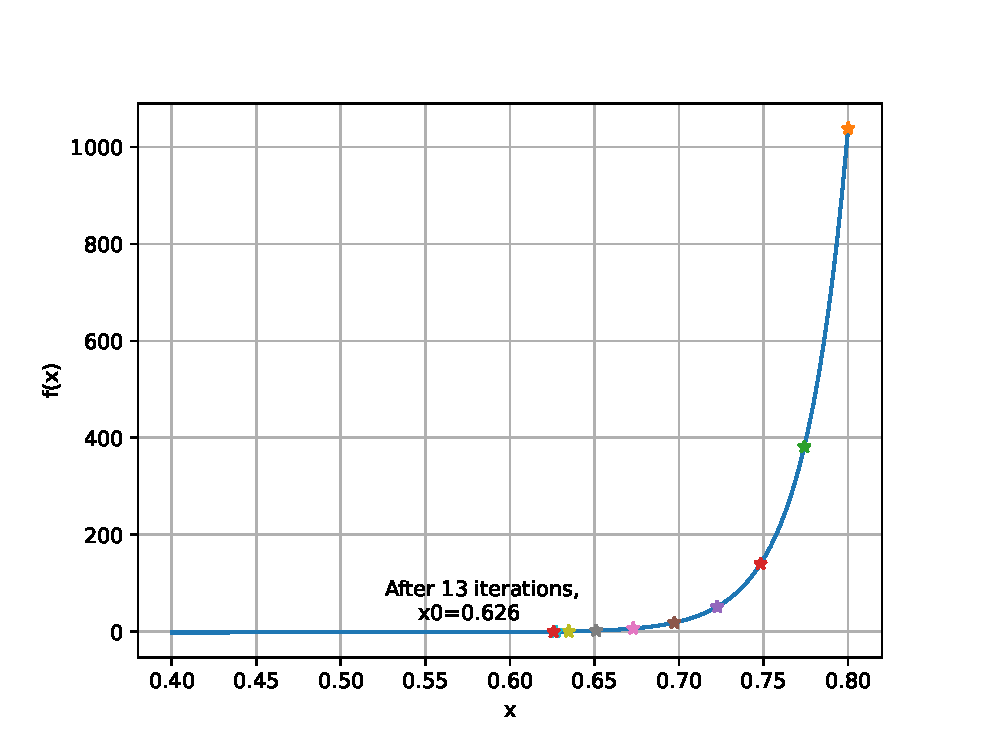
\includegraphics[scale=0.5]{./figs/Q2_solv.eps}\\
 \newline
Verifying the solution $V_D=0.626V$,\\
\begin{gather*}
4000*I_s\left(e^{\frac{V_D}{V_T}} - 1\right) + 2V_D -2.5 = -8.88E-16 \approx 0\\
\implies I_D = 312{\mu}A
\end{gather*}
\subsection*{(c)}
\textbf{Netlist}\\
\begin{lstlisting}
V1 N001 0 2.5
R1 N002 N001 2k
D1 N002 N003 ideal_diode
R2 N003 N004 2k
D2 N004 0 ideal_diode
.model D D
.lib C:\users\solomon\My Documents\LTspiceXVII\lib\cmp\standard.dio
.model ideal_diode D (IS=0.01p)
.tran 10m
.backanno
.end
\end{lstlisting}
\textbf{Testbench}\\
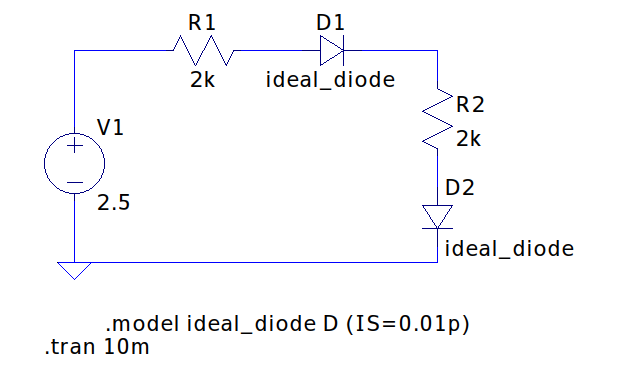
\includegraphics[scale=0.5]{./figs/Q2_tb.png}\\
 \newline
\textbf{Current}\\
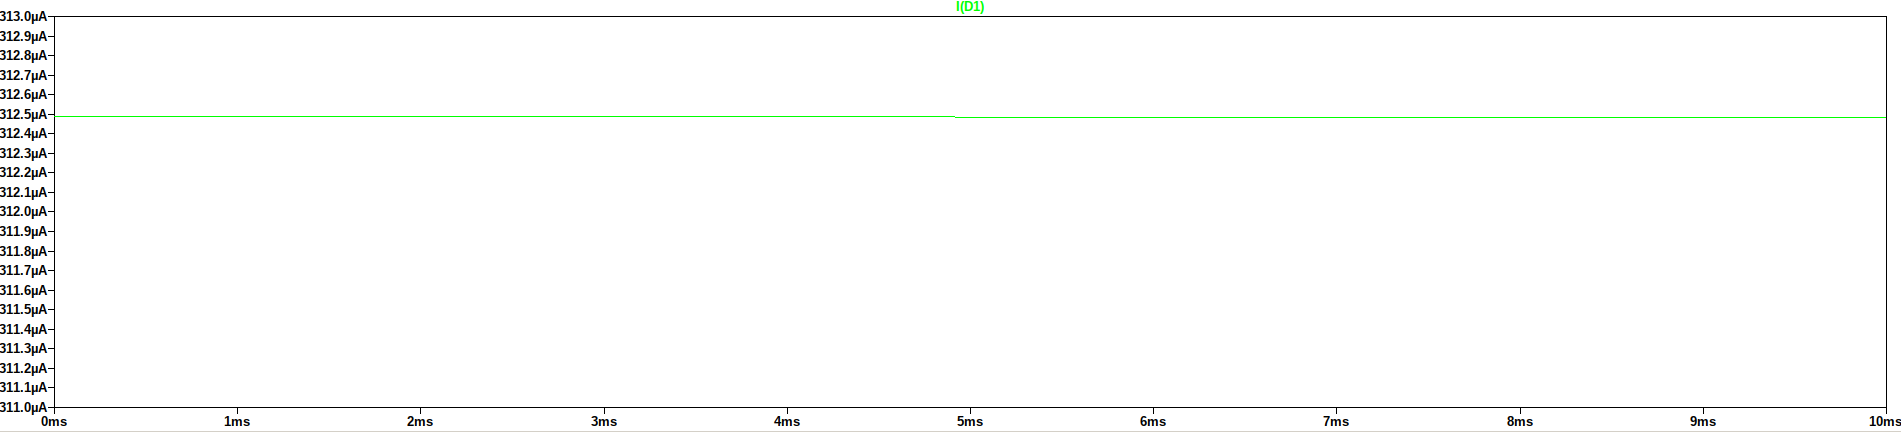
\includegraphics[scale=0.28]{./figs/Q2_c_i.png}
 \newline
\textbf{Voltage}\\
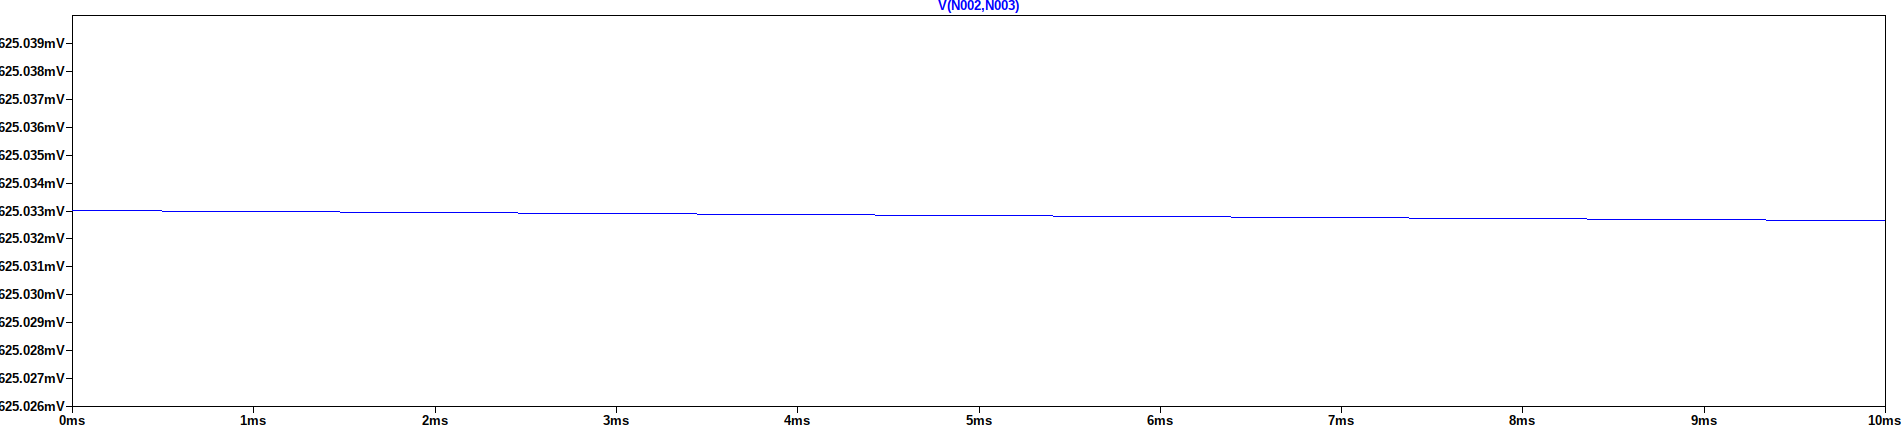
\includegraphics[scale=0.28]{./figs/Q2_c_v.png}
 \newline
\textbf{Comparisions}\\
\begin{center}
\begin{tabular}{|c|c|c|}
\hline
\textbf{Question} & $\mathbf{I_D}$ & $\mathbf{V_D}$ \\
\hline
(a) & 275$\mu$A & 0.7V\\
\hline
(b) & 312$\mu$A & 0.626V\\
\hline
(c) & 312.5$\mu$A & 0.625V\\
\hline
\end{tabular}
\end{center}

\section{Controlled sources}
\textbf{SPICE Netlist}
\begin{lstlisting}
Vin 0 N002 SINE(0 0.5 1k)
R1 N001 N002 1k
G1 0 Out N001 0 1Mega
R2 Out N001 3k
R3 Out 0 1
.tran 10m
.backanno
.end
\end{lstlisting}
\textbf{TestBench}\\
\includegraphics[scale=0.5]{./figs/Q3_tb.png}\\
\textbf{Output Response}\\
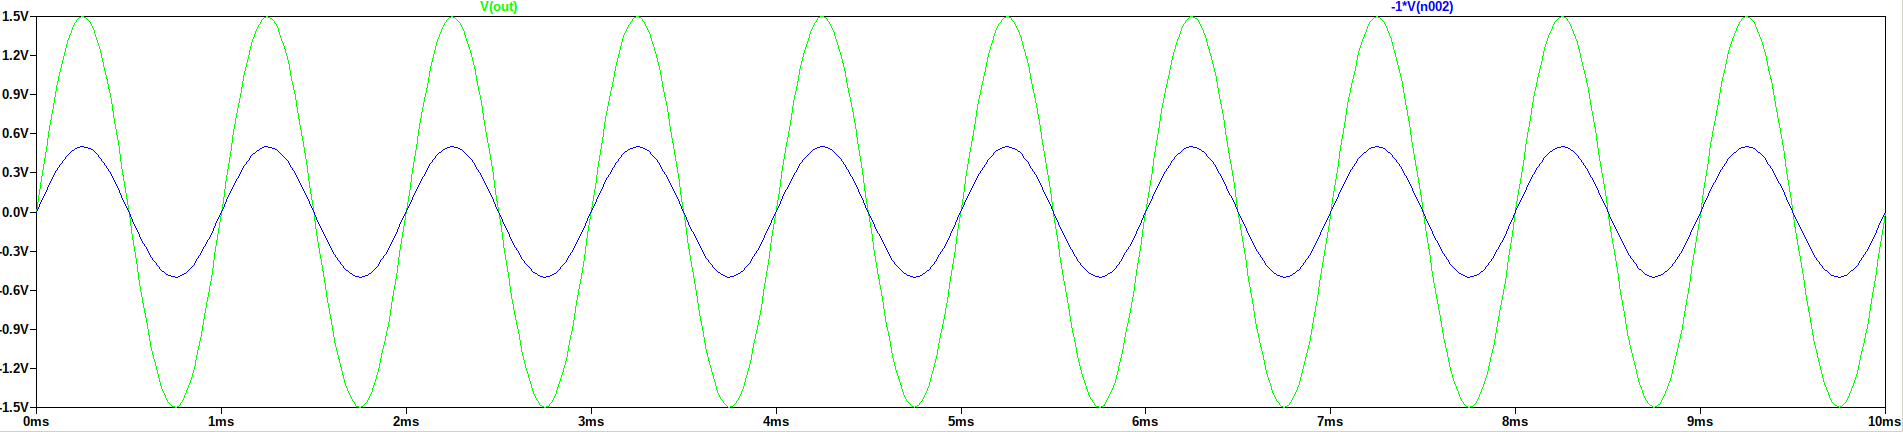
\includegraphics[scale=0.28]{./figs/Q3_sr.png}\\
\textbf{Gain}\\
\includegraphics[scale=0.5]{./figs/Q3_re.png}\\
\begin{equation*}
\tcbhighmath[drop fuzzy shadow]{\frac{v_{out}}{v_{in}} = 3}
\end{equation*}
\textbf{Analytical solution},\\
VCCS has very high gain which means that both the teriminal of voltage taps will be approximalty same inorder to make current flow zero else there would very high current flow.\\
\begin{gather*}
-v_{in} -1000i = 0 \implies i = \frac{-v_{in}}{1000}\\
v_{out} = 0 - 3000*i\\
\implies \frac{v_{out}}{v_{in}} = 3
\end{gather*}

\section{MOSFET Characteristics}
\subsection{NMOS}
\textbf{Short Channel}\\
\textbf{SPICE Netlist}
\begin{lstlisting}
* Z:\home\solomon\VLSI\Assignments\Assignment 1\Simulation\Q4_nmos_sc.asc
Vgs N002 0 {Vgs}
M1 N001 N002 0 0 nch_tt l=180n w=270n
Vds N001 0 1.8
.model NMOS NMOS
.model PMOS PMOS
.lib C:\users\solomon\My Documents\LTspiceXVII\lib\cmp\standard.mos
.include TSMC180.lib
.step param Vgs list 0.4 0.5 0.6 0.7 0.8 0.9
.dc Vds 0 1.8 1m
;.dc Vgs 0 1.8
* Short Channel
* W = 270nm, L = 180nm
.backanno
.end
\end{lstlisting}
\textbf{TestBench}\\
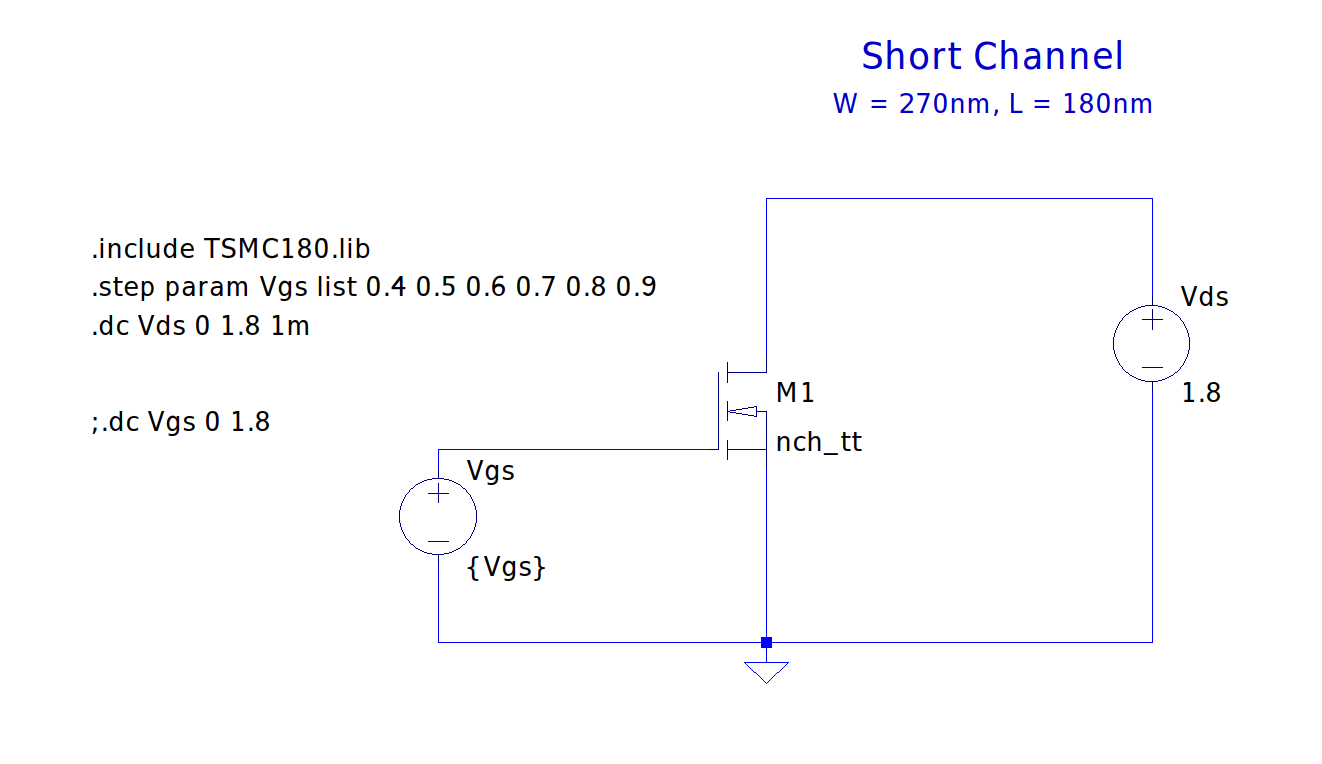
\includegraphics[scale=0.28]{./figs/Q4_nmos_sc_tb.png}\\
 \newline
\textbf{Long Channel}\\
\textbf{SPICE Netlist}
\begin{lstlisting}
* Z:\home\solomon\VLSI\Assignments\Assignment 1\Simulation\Q4_nmos_lc.asc
Vgs N002 0 {Vgs}
M1 N001 N002 0 0 nch_tt l=10u w=15u
Vds N001 0 1.8
.model NMOS NMOS
.model PMOS PMOS
.lib C:\users\solomon\My Documents\LTspiceXVII\lib\cmp\standard.mos
.include TSMC180.lib
.step param Vgs list 0.4 0.5 0.6 0.7 0.8 0.9
.dc Vds 0 1.8 1m
;.dc Vgs 0 0.4
* Long Channel
* W = 15um, L = 10um
.backanno
.end
\end{lstlisting}
\textbf{TestBench}\\
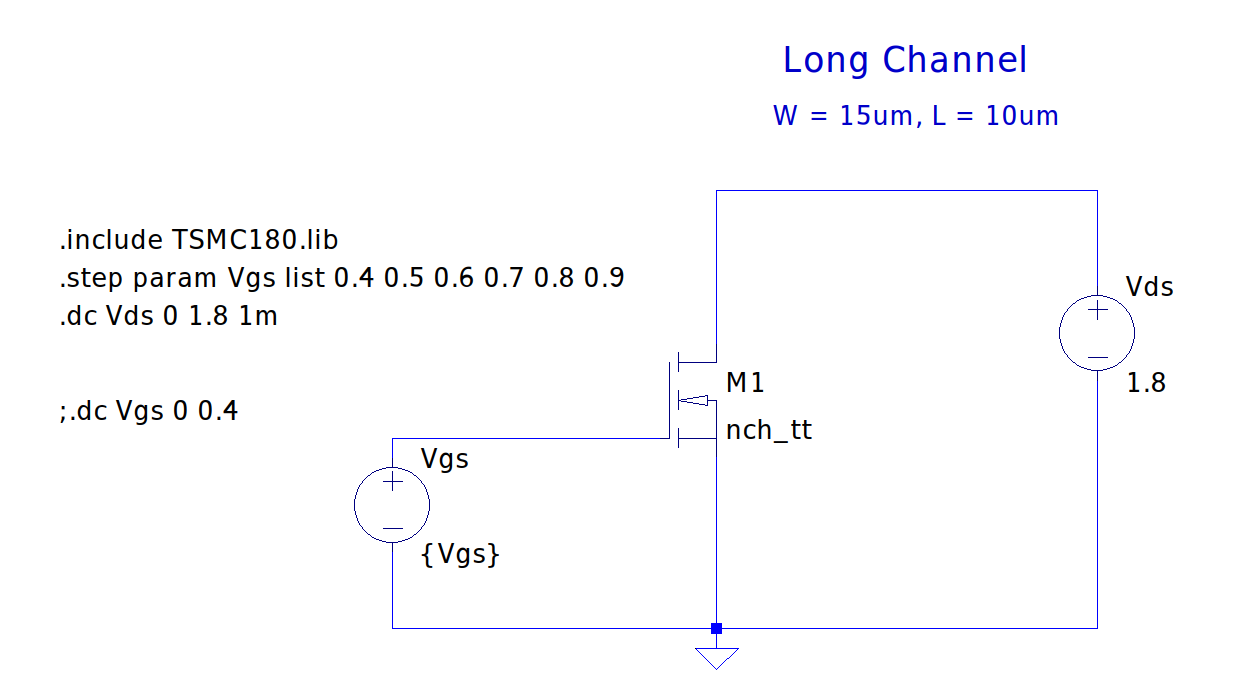
\includegraphics[scale=0.28]{./figs/Q4_nmos_lc_tb.png}\\

\subsubsection*{(a)}
\textbf{$I_{ds}$ vs $V_{ds}$}\\
 \newline
\textbf{Short Channel}\\
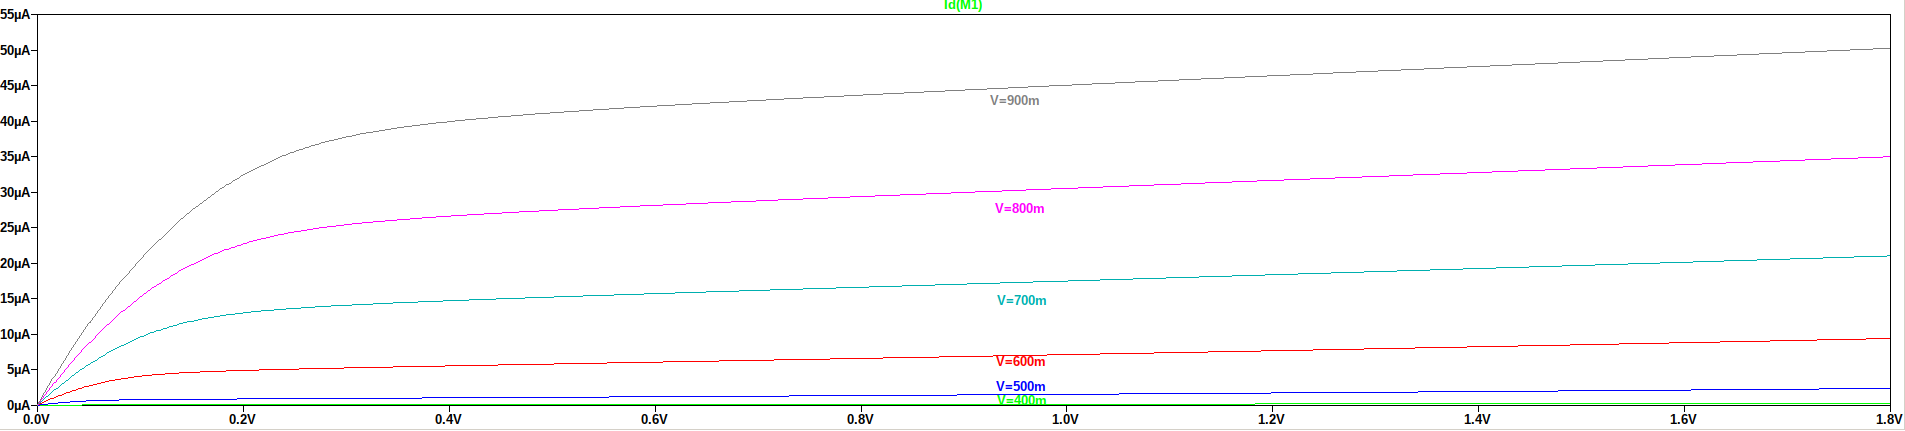
\includegraphics[scale=0.28]{./figs/Q4_a_nmos_sc_vds.png}\\
 \newline
\textbf{Long Channel}\\
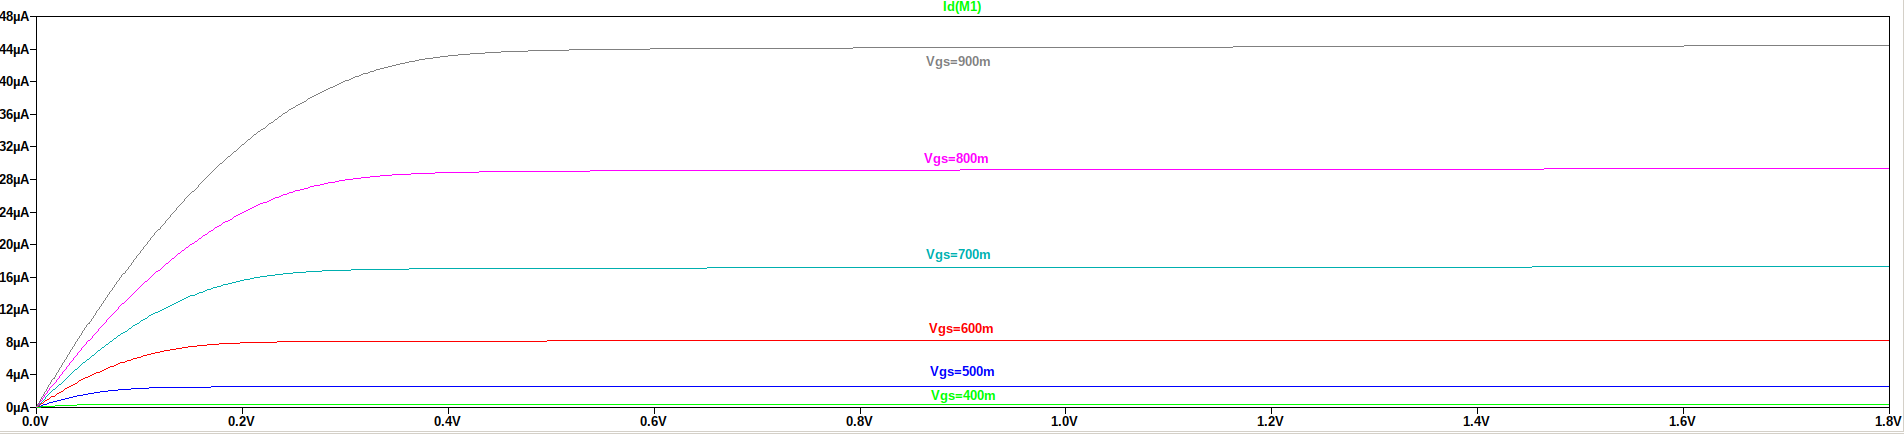
\includegraphics[scale=0.28]{./figs/Q4_a_nmos_lc_vds.png}
 \newline
 \newline
\textbf{$I_{ds}$ vs $V_{gs}$}\\
 \newline
\textbf{Short Channel}\\
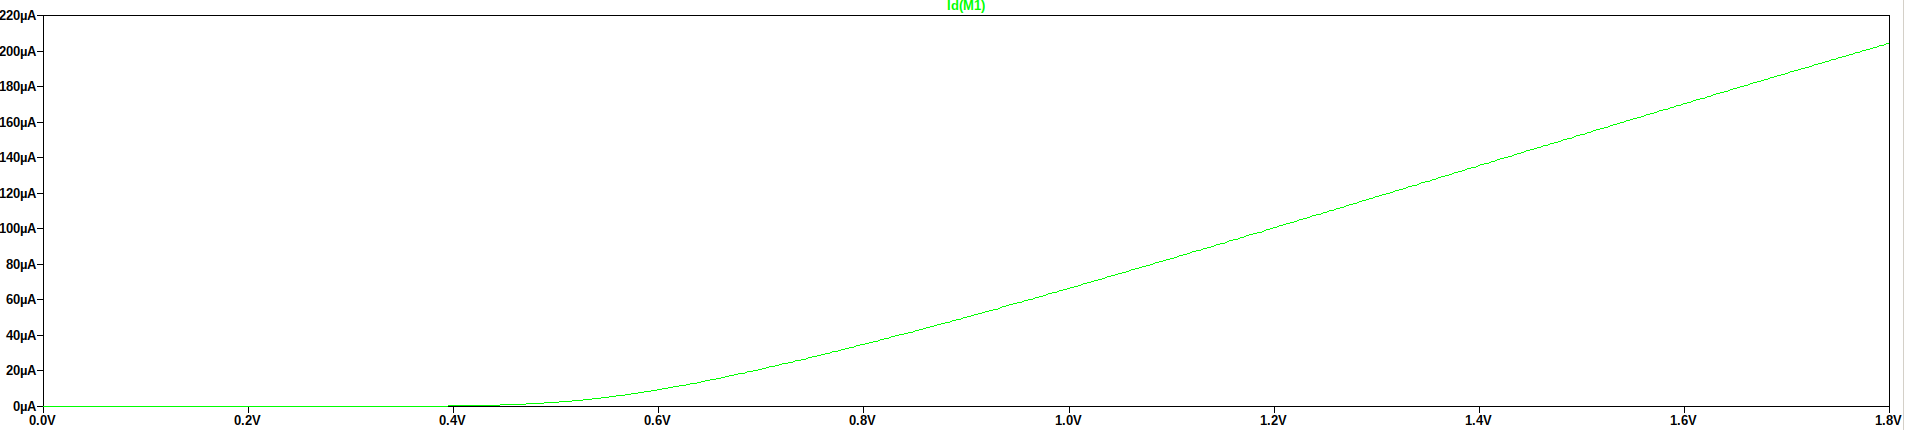
\includegraphics[scale=0.28]{./figs/Q4_a_nmos_sc_vgs.png}\\
 \newline
\textbf{Long Channel}\\
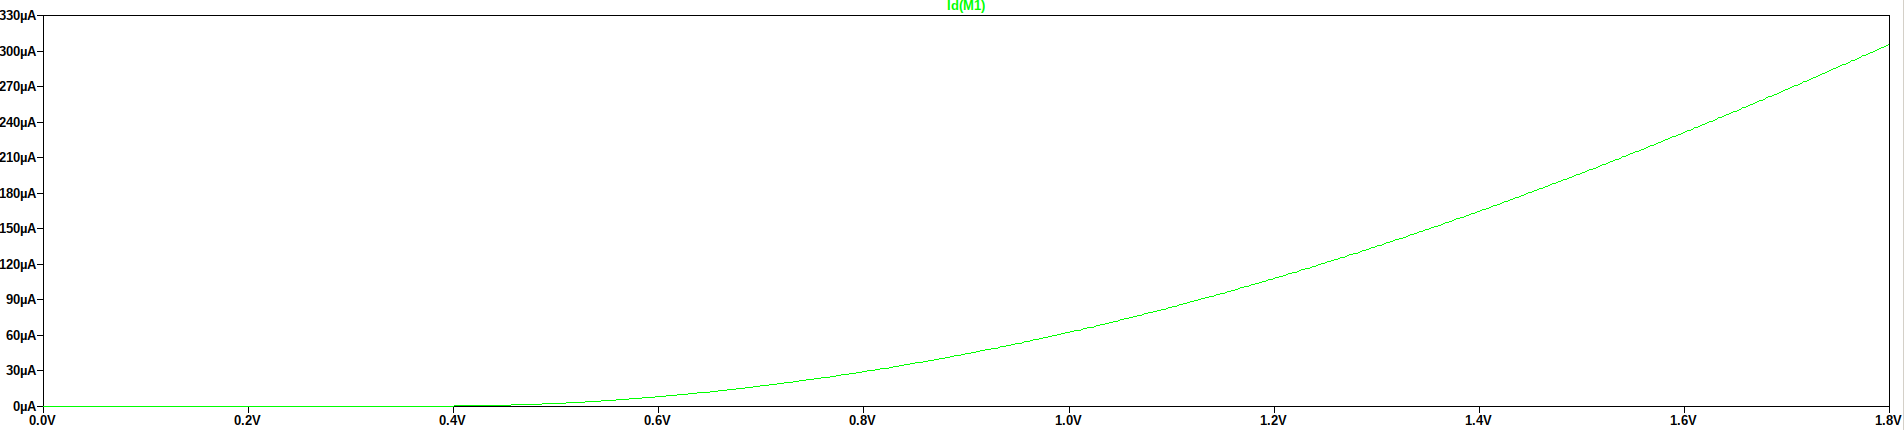
\includegraphics[scale=0.28]{./figs/Q4_a_nmos_lc_vgs.png}

\subsubsection*{(b)}
\textbf{$I_{ds}$ vs $V_{ds}$}\\
 \newline
\textbf{Short Channel}\\
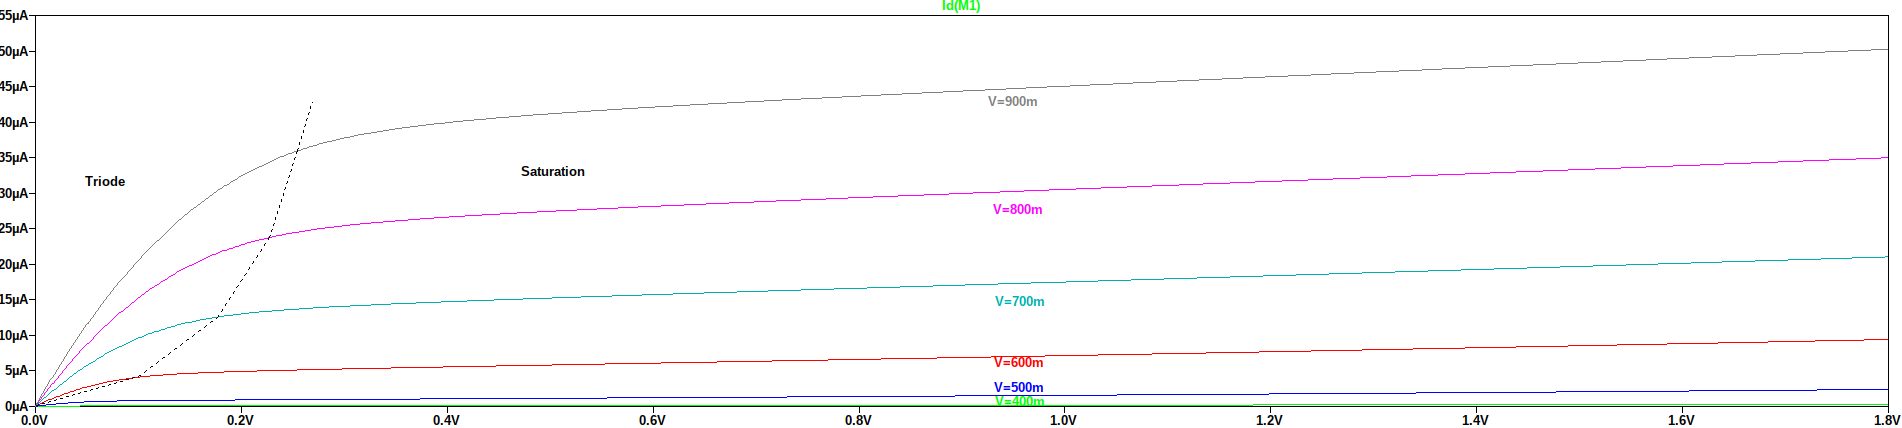
\includegraphics[scale=0.28]{./figs/Q4_b_nmos_sc.png}\\
 \newline
\textbf{Long Channel}\\
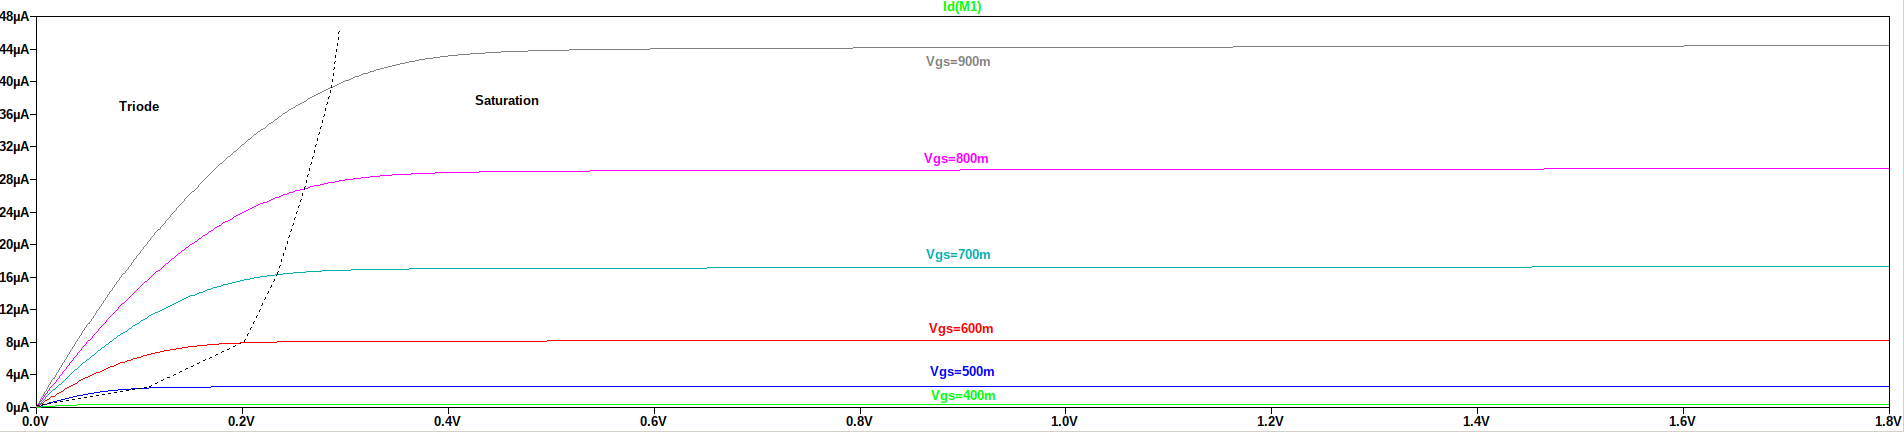
\includegraphics[scale=0.28]{./figs/Q4_b_nmos_lc.png}\\
 \newline
\textbf{Differences}\\
Current in saturation of short channel MOSFET is not constant but has a linear dependency on $V_{ds}$, which is also known as \textbf{Channel length modulation}. This effect is significant in shorter channel devices as decrement of channel length in shorter channel is significant compared to longer length channel due to delpletion regions formed at higher $V_{ds}$. 
\subsubsection*{(c)}
In $I_{ds}$ vs $V_{ds}$ characteristics, the below graphs are obtained by taking $\frac{1}{\frac{\partial i_{ds}}{\partial v_{ds}}}$.\\
\textbf{Short Channel}\\
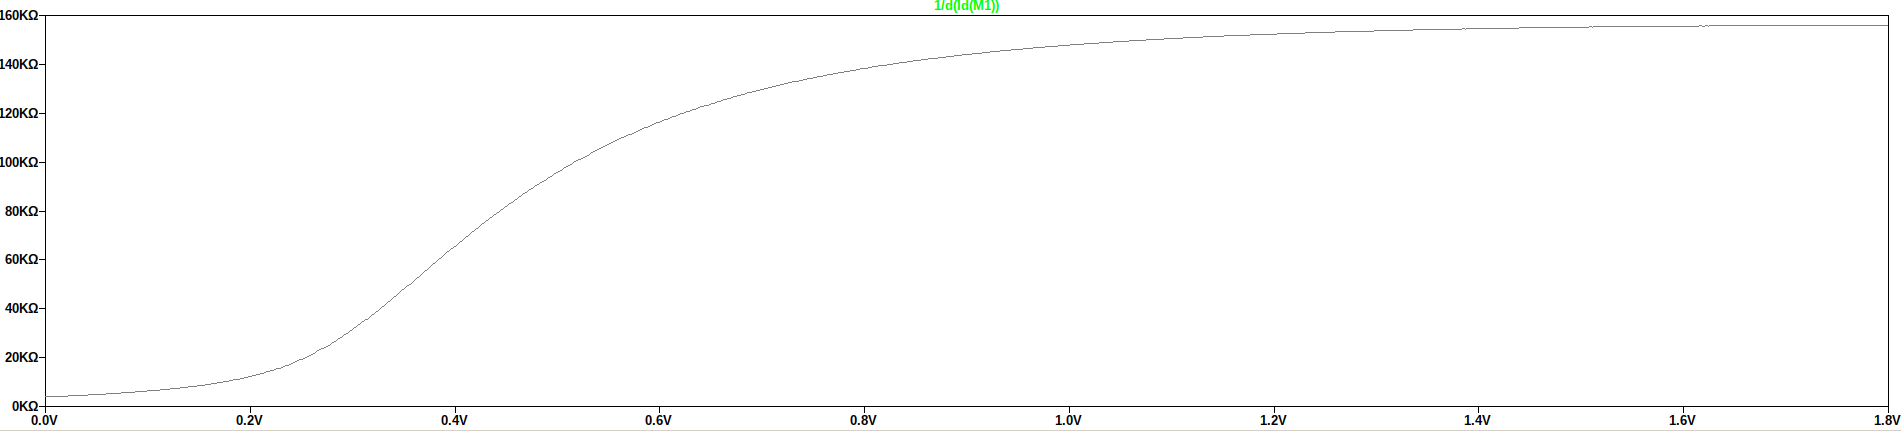
\includegraphics[scale=0.28]{./figs/Q4_nmos_sc_c.png}\\
It is observed that small signal output resistance is \textbf{155.65k$\si{\ohm}$}.\\
 \newline
\textbf{Long Channel}\\
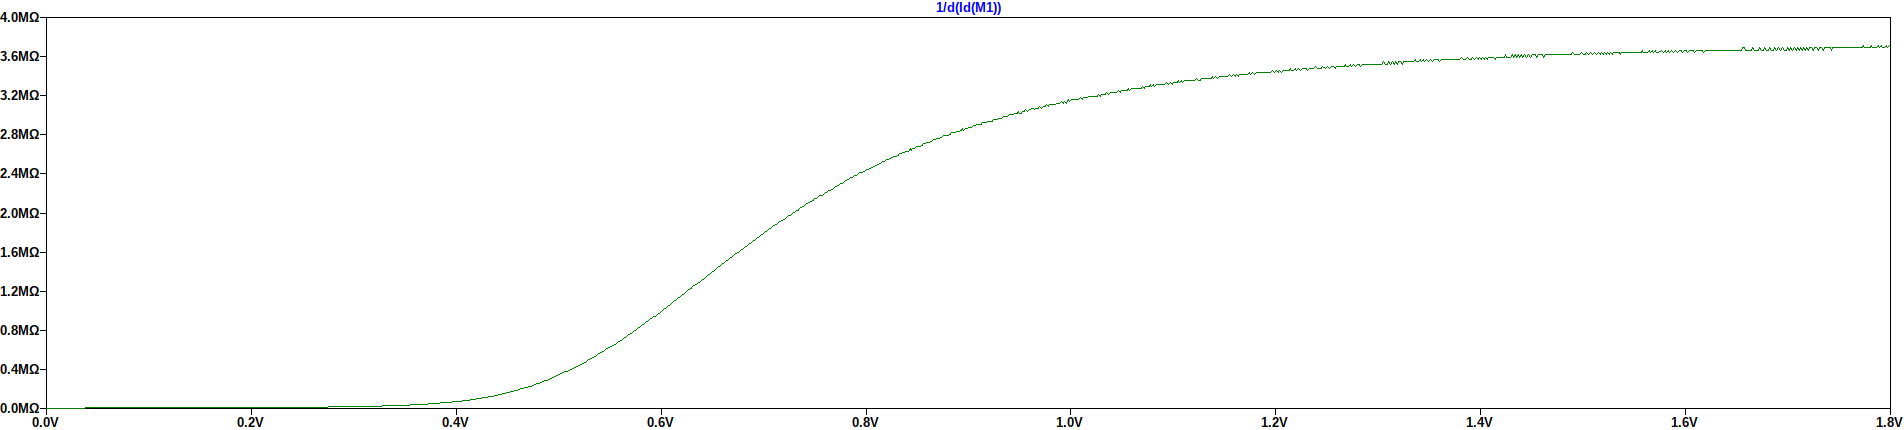
\includegraphics[scale=0.28]{./figs/Q4_nmos_lc_c.png}\\
It is observed that small signal output resistance is \textbf{3.66M$\si{\ohm}$}.

\subsubsection*{(d)}
\textbf{Short Channel}\\
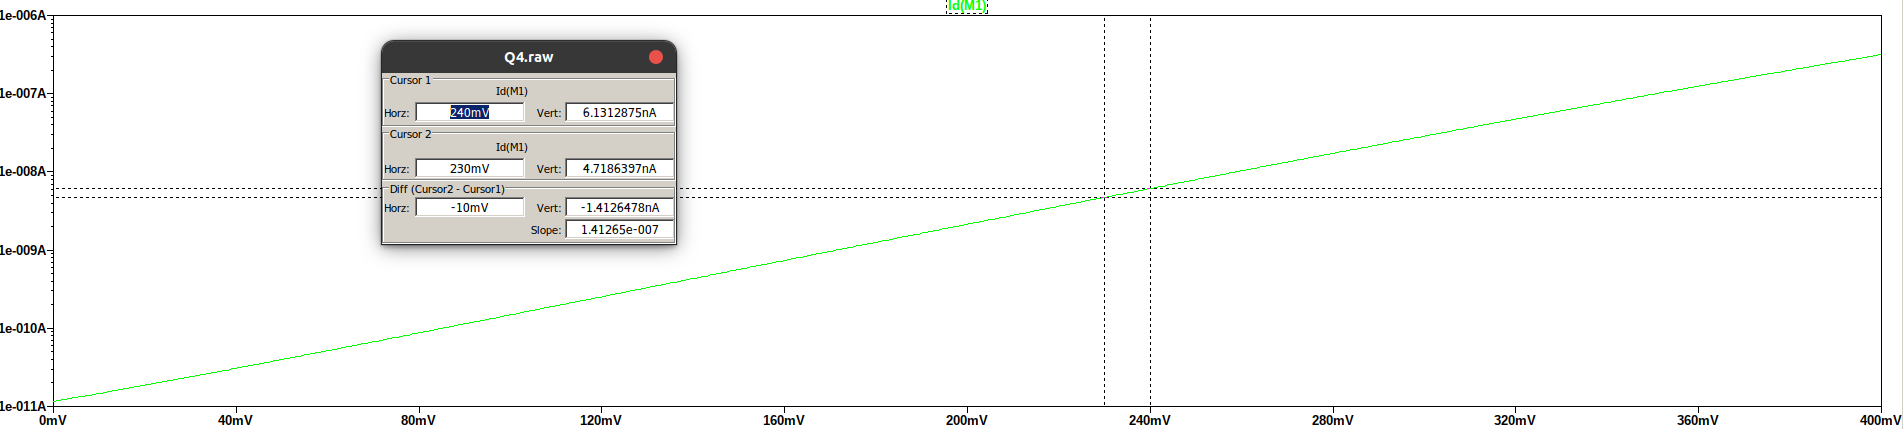
\includegraphics[scale=0.28]{./figs/Q4_b_sc_st.png}\\
Slope = 1.41265x$10^{-7}$
\begin{gather*}
S = n\left(\frac{kT}{q}\right)ln(10) = 1.41265e-7
\implies \tcbhighmath[drop fuzzy shadow]{n = 2.368x10^{-6}}
\end{gather*}
 \newline
\textbf{Long Channel}\\
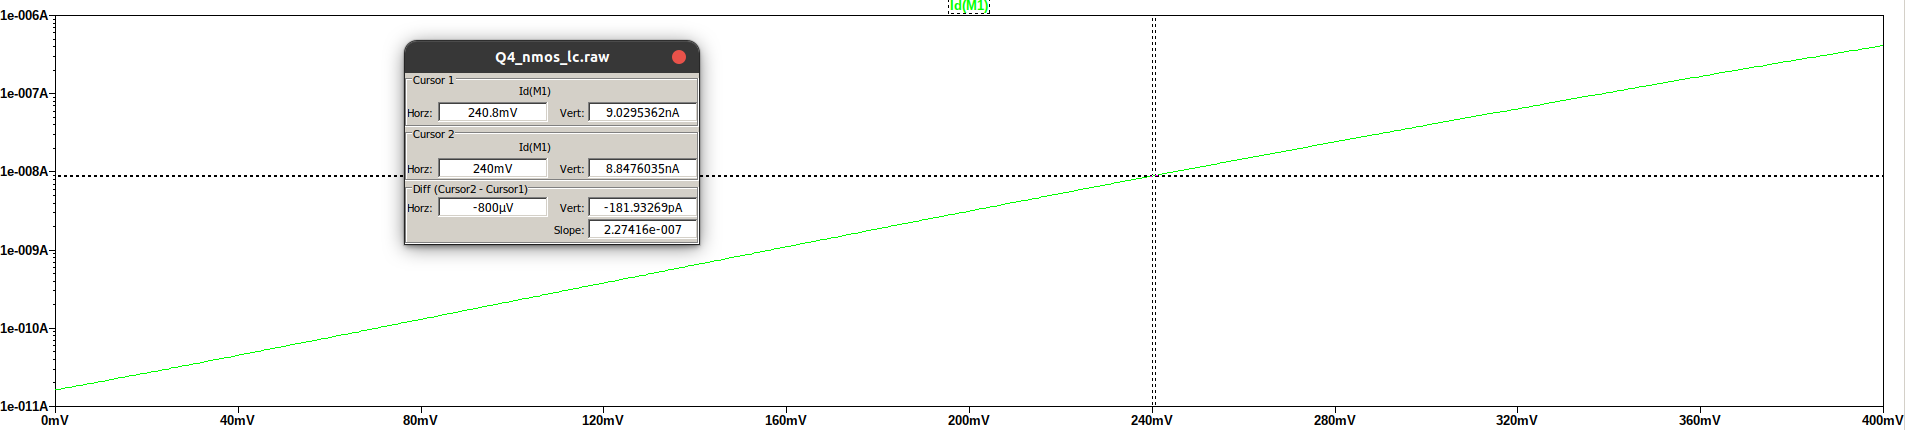
\includegraphics[scale=0.28]{./figs/Q4_b_nmos_lc_vgs_st.png}
Slope = 2.27416x$10^{-7}$
\begin{gather*}
S = n\left(\frac{kT}{q}\right)ln(10) = 2.27416e-7
\implies \tcbhighmath[drop fuzzy shadow]{n = 3.8133x10^{-6}}
\end{gather*}	

\subsection{PMOS}
\textbf{Short Channel}\\
\textbf{SPICE Netlist}
\begin{lstlisting}
* Z:\home\solomon\VLSI\Assignments\Assignment 1\Simulation\Q4_pmos_sc.asc
Vsd N001 0 1.8
M1 0 N002 N001 N001 pch_tt L = 180n W = 270n
Vsg N001 N002 {Vsg}
.model NMOS NMOS
.model PMOS PMOS
.lib C:\users\solomon\My Documents\LTspiceXVII\lib\cmp\standard.mos
.include TSMC180.lib
.step param Vsg list 0.4 0.5 0.6 0.7 0.8 0.9
.dc Vsd 0 1.8 1m
;.dc Vsg 0 1.8 1m
* Short Channel
* W = 270nm, L = 180nm
.backanno
.end
\end{lstlisting}
\textbf{TestBench}\\
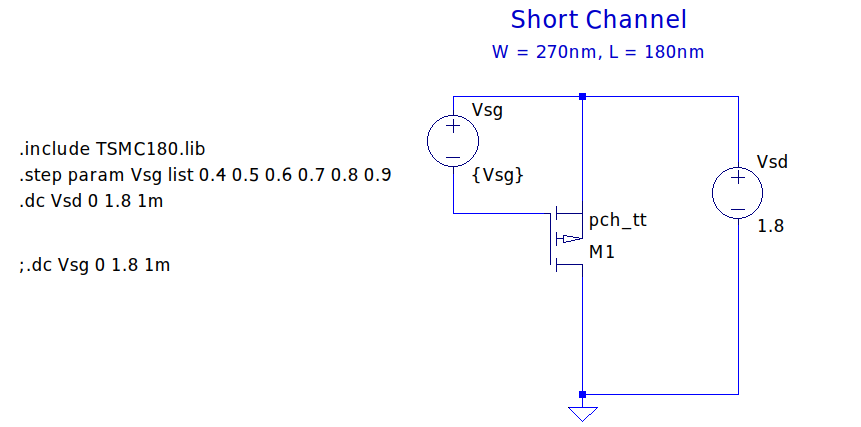
\includegraphics[scale=0.4]{./figs/Q4_pmos_sc_tb.png}\\
 \newline
\textbf{Long Channel}\\
\textbf{SPICE Netlist}
\begin{lstlisting}
* Z:\home\solomon\VLSI\Assignments\Assignment 1\Simulation\Q4_pmos_lc.asc
Vsd N001 0 1.8
M1 0 N002 N001 N001 pch_tt L = 10u W = 15u
Vsg N001 N002 0.9
.model NMOS NMOS
.model PMOS PMOS
.lib C:\users\solomon\My Documents\LTspiceXVII\lib\cmp\standard.mos
.include TSMC180.lib
.step param Vsg list 0.4 0.5 0.6 0.7 0.8 0.9
.dc Vsd 0 1.8 1m
;.dc Vsg 0 1.8 1m
* Long Channel
* W = 15u, L = 10u
.backanno
.end
\end{lstlisting}
\textbf{TestBench}\\
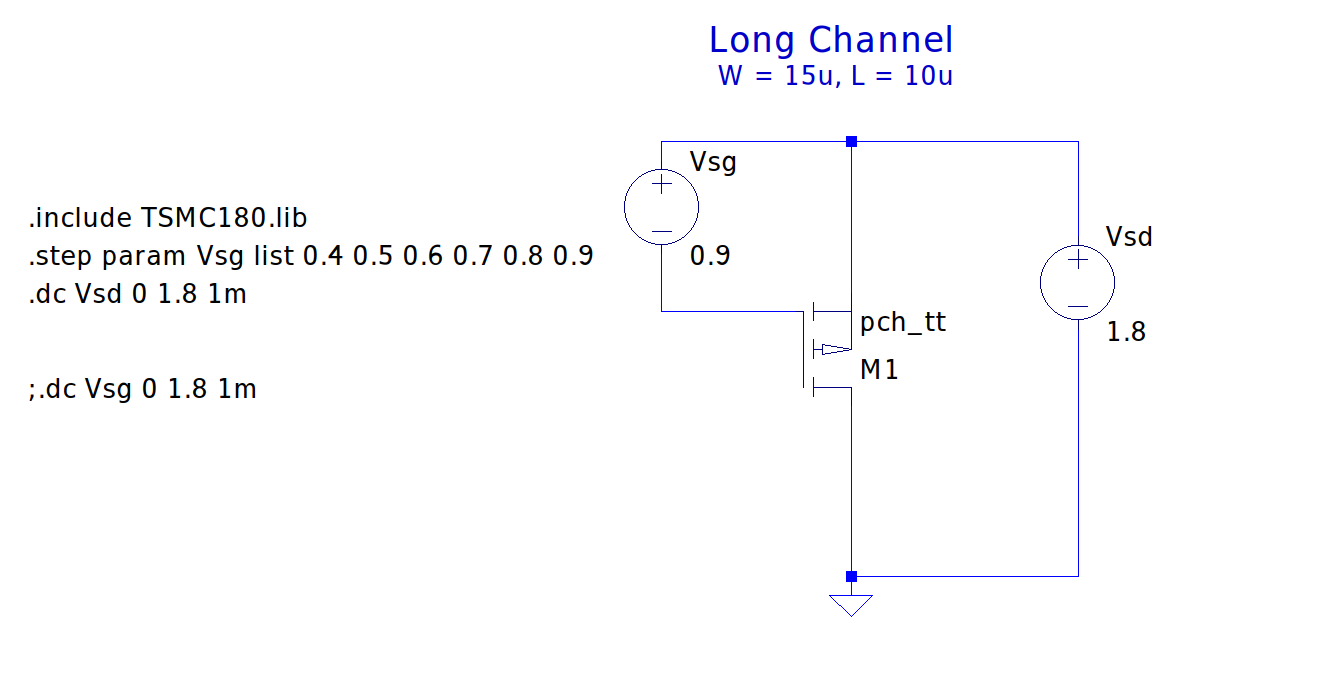
\includegraphics[scale=0.28]{./figs/Q4_pmos_lc_tb.png}\\

\subsubsection*{(a)}
\textbf{$I_{ds}$ vs $V_{ds}$}\\
 \newline
\textbf{Short Channel}\\
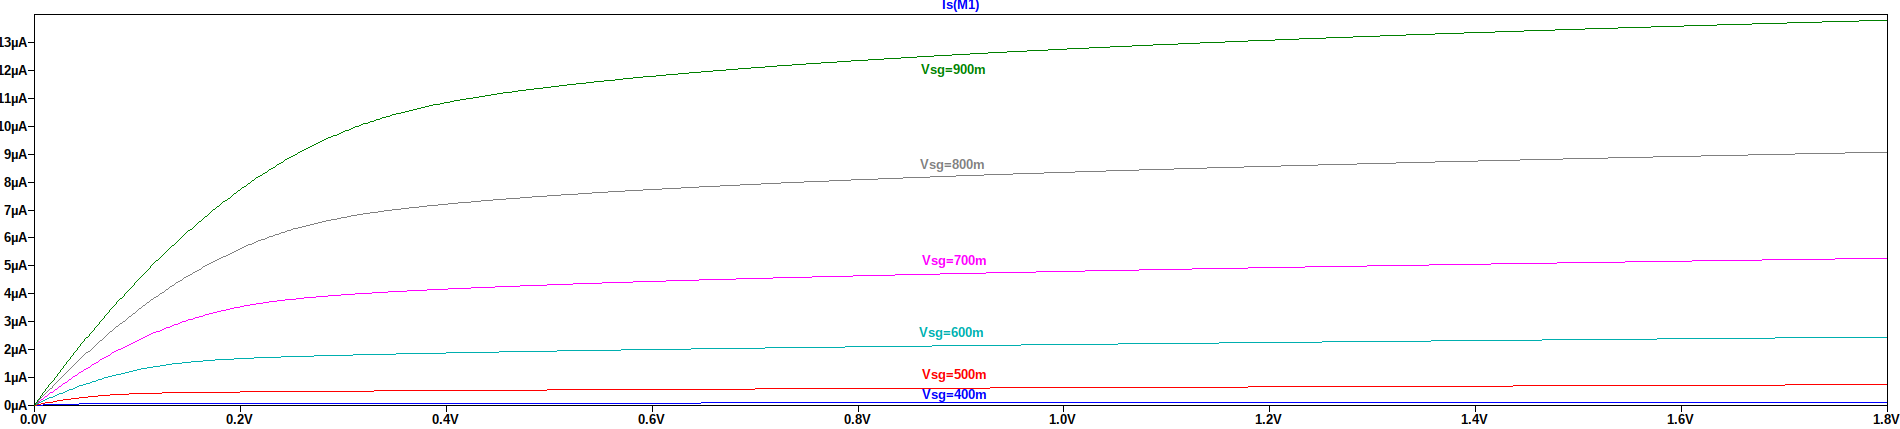
\includegraphics[scale=0.28]{./figs/Q4_pmos_sc_vds.png}\\
 \newline
\textbf{Long Channel}\\
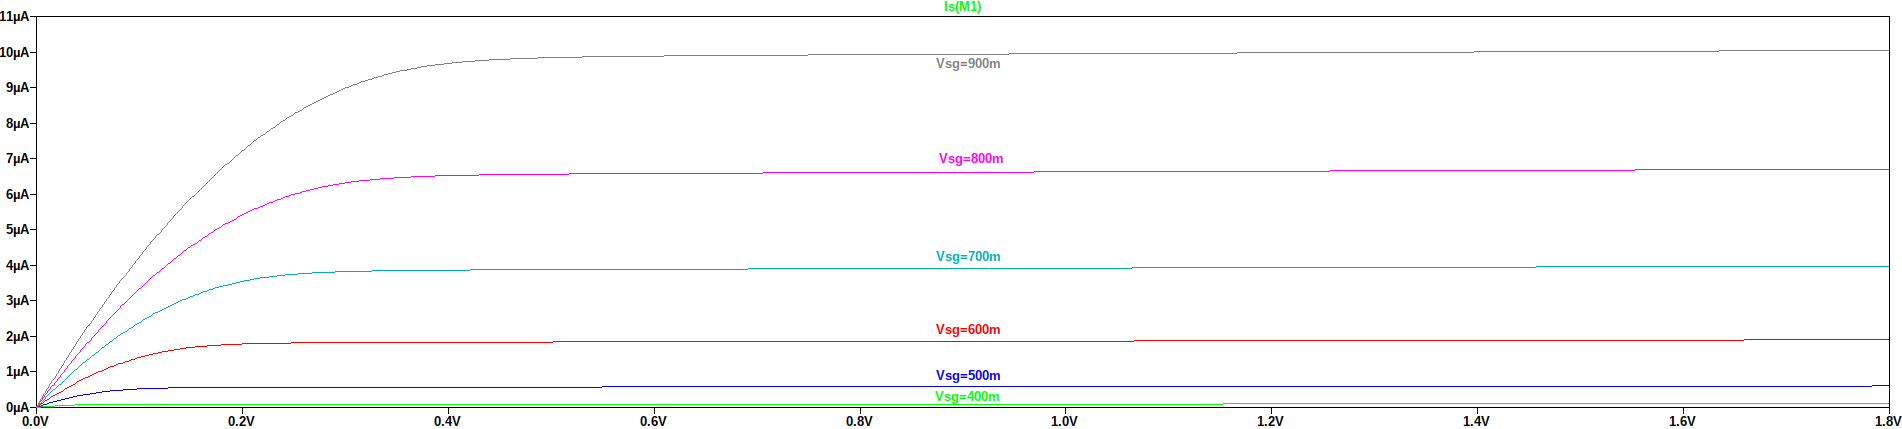
\includegraphics[scale=0.28]{./figs/Q4_pmos_lc_vds.png}
 \newline
 \newline
\textbf{$I_{ds}$ vs $V_{gs}$}\\
 \newline
\textbf{Short Channel}\\
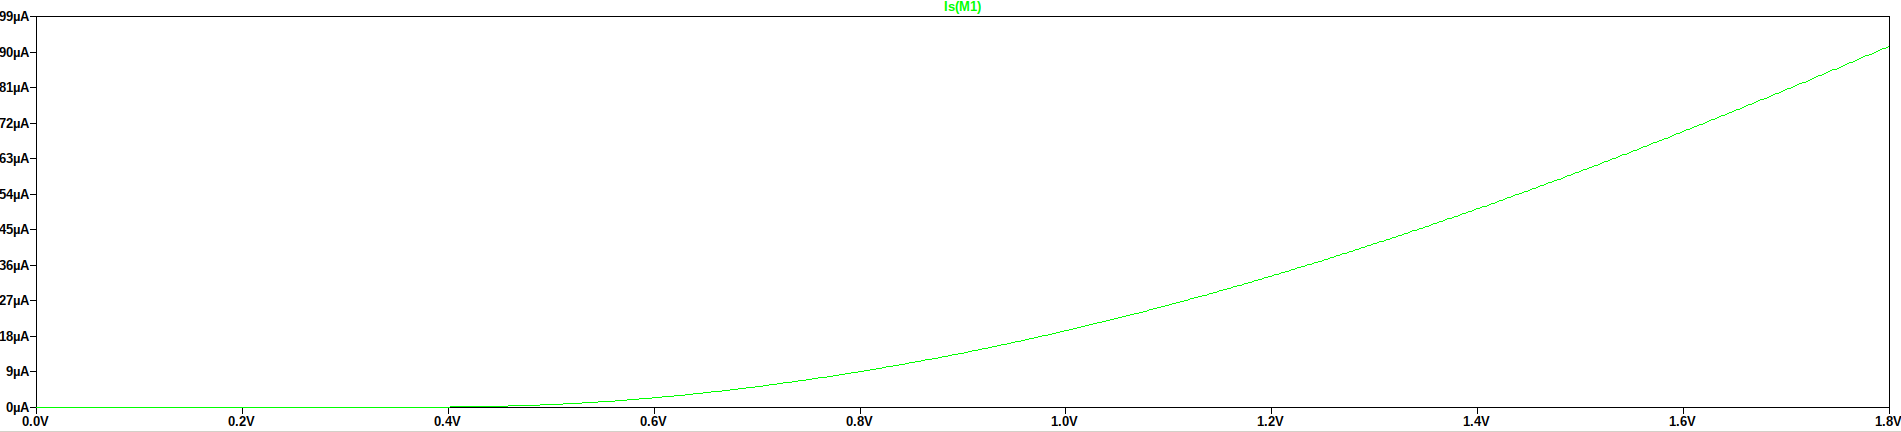
\includegraphics[scale=0.28]{./figs/Q4_pmos_sc_vgs.png}\\
 \newline
\textbf{Long Channel}\\
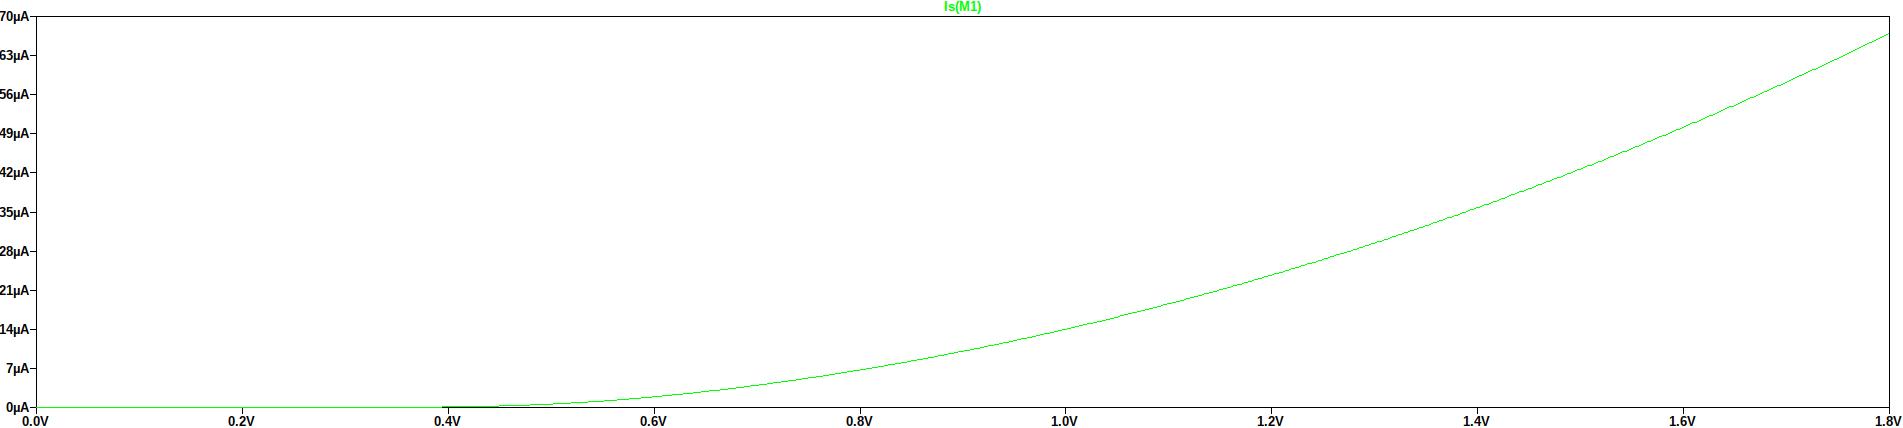
\includegraphics[scale=0.28]{./figs/Q4_pmos_lc_vgs.png}

\subsubsection*{(b)}
\textbf{$I_{ds}$ vs $V_{ds}$}\\
 \newline
\textbf{Short Channel}\\
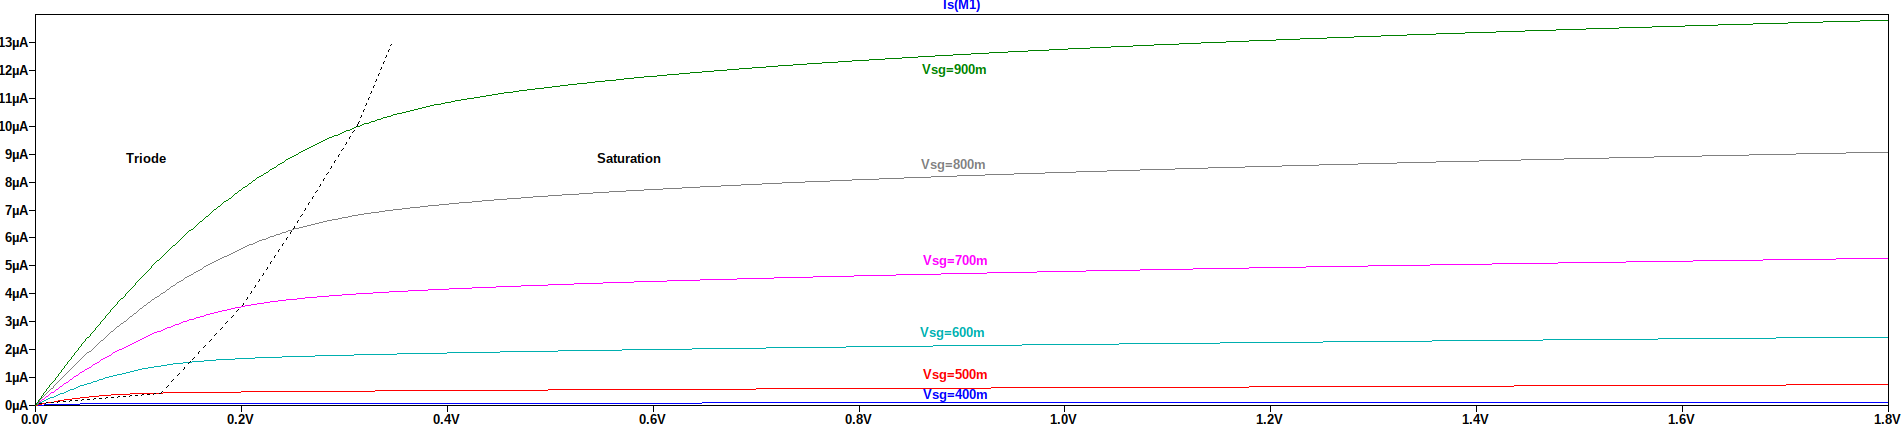
\includegraphics[scale=0.28]{./figs/Q4_pmos_sc_vds_st.png}\\
 \newline
\textbf{Long Channel}\\
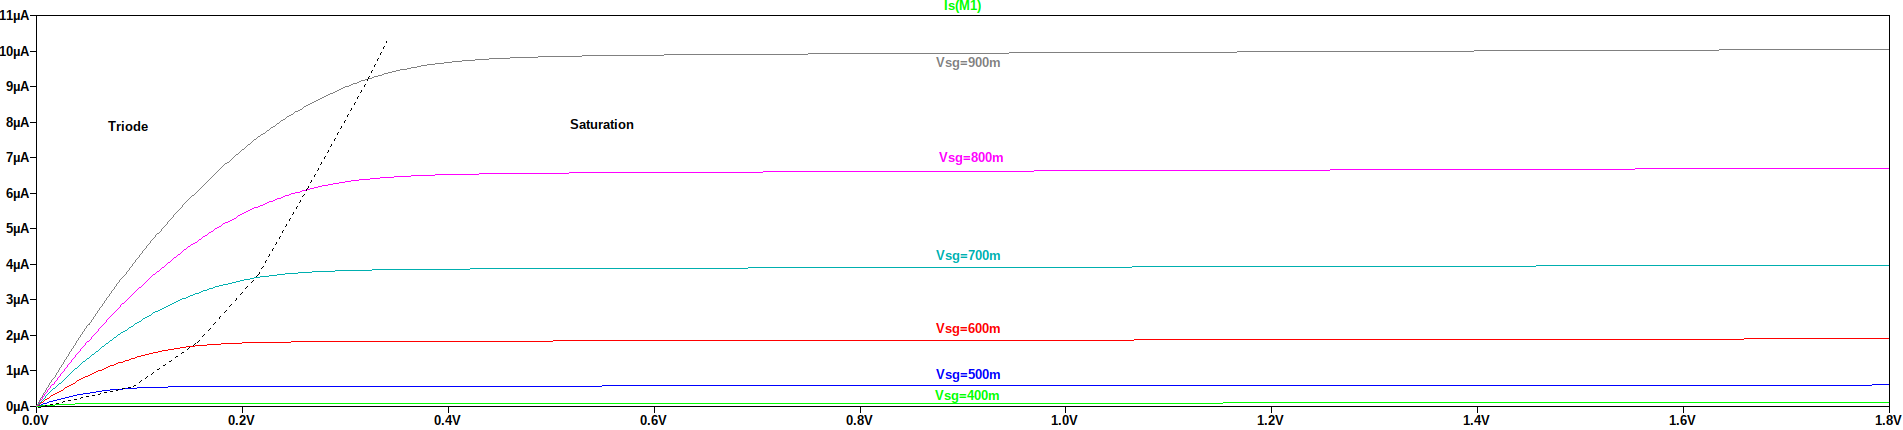
\includegraphics[scale=0.28]{./figs/Q4_pmos_lc_vds_st.png}\\
 \newline
\textbf{Differences}\\
Current in saturation of short channel MOSFET is not constant but has a linear dependency on $V_{ds}$, which is also known as \textbf{Channel length modulation}. This effect is significant in shorter channel devices as decrement of channel length in shorter channel is significant compared to longer length channel due to delpletion regions formed at higher $V_{ds}$. 

\subsubsection*{(c)}
In $I_{sd}$ vs $V_{sd}$ characteristics, the below graphs are obtained by taking $\frac{1}{\frac{\partial i_{sd}}{\partial v_{sd}}}$.\\
\textbf{Short Channel}\\
\includegraphics[scale=0.28]{./figs/Q4_pmos_sc_c.png}\\
It is observed that small signal output resistance is \textbf{1.1M$\si{\ohm}$}.\\
 \newline
\textbf{Long Channel}\\
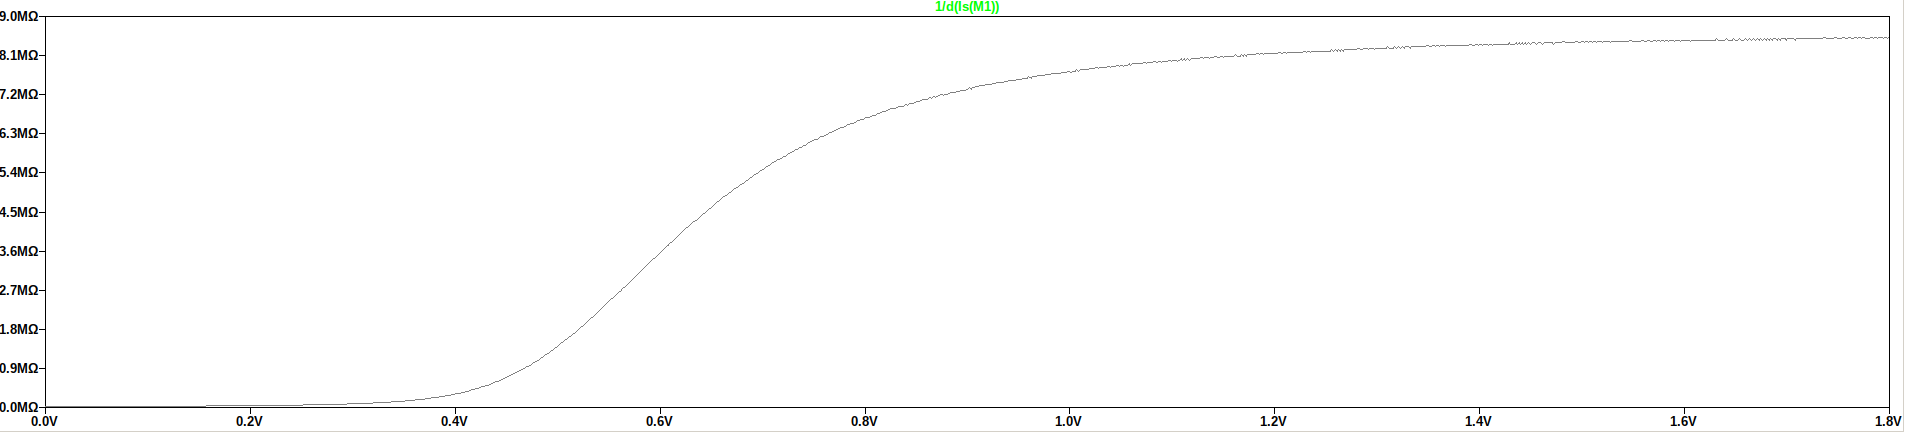
\includegraphics[scale=0.28]{./figs/Q4_pmos_lc_c.png}\\
It is observed that small signal output resistance is \textbf{8.51M$\si{\ohm}$}.

\subsubsection*{(d)}
\textbf{Short Channel}\\
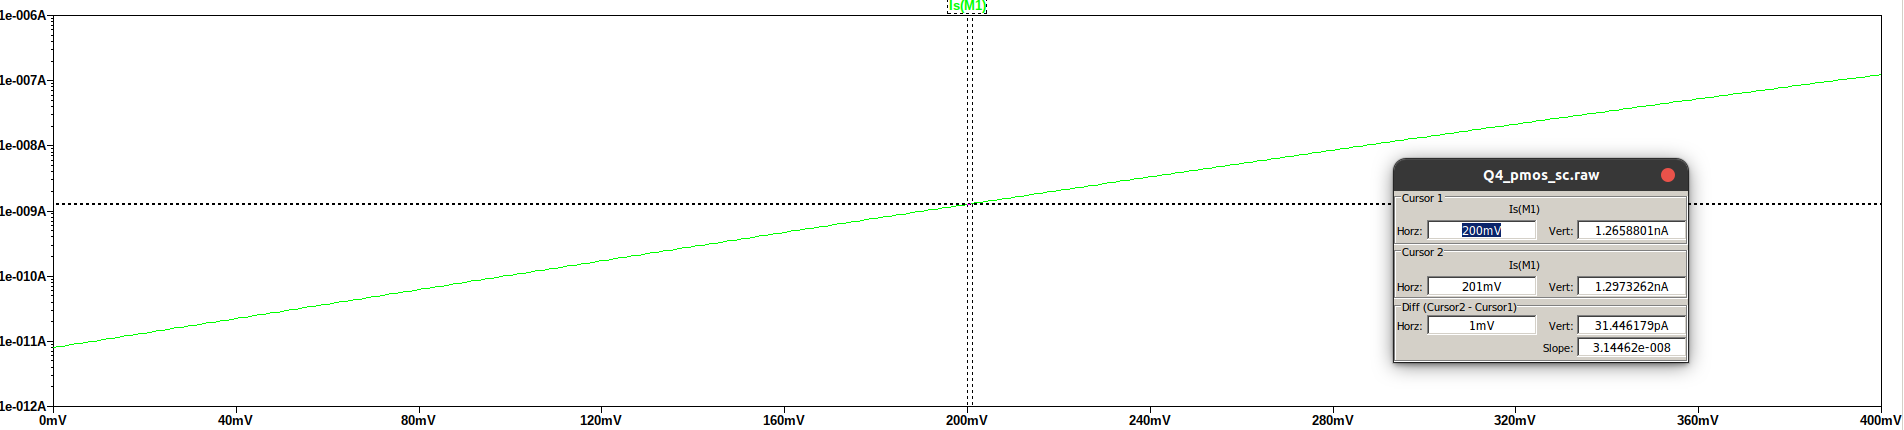
\includegraphics[scale=0.28]{./figs/Q4_pmos_sc_sub.png}\\
Slope = 1.41265x$10^{-8}$
\begin{gather*}
S = n\left(\frac{kT}{q}\right)ln(10) = 1.41265e-8
\implies \tcbhighmath[drop fuzzy shadow]{n = 5.454x10^{-7}}
\end{gather*}
 \newline
\textbf{Long Channel}\\
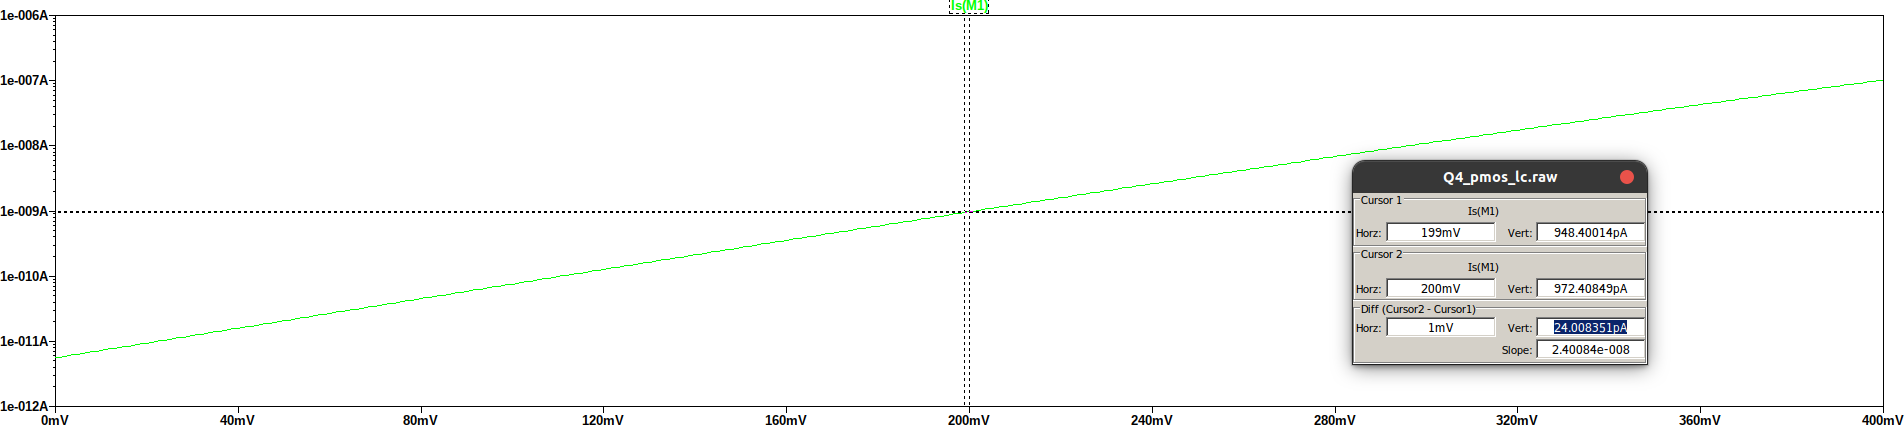
\includegraphics[scale=0.28]{./figs/Q4_pmos_lc_sub.png}
Slope = 3.144x$10^{-8}$
\begin{gather*}
S = n\left(\frac{kT}{q}\right)ln(10) = 3.144e-8
\implies \tcbhighmath[drop fuzzy shadow]{n = 1.214x10^{-6}}
\end{gather*}		

\subsection*{Final comparisions}
\textbf{Output Resistances}
\begin{center}
\begin{tabular}{|c|c|c|}
\hline
\textbf{Device} & $\mathbf{\frac{W}{L}}$ \textbf{= 1.5} & $\mathbf{r_o}$ \\
\hline
\multirow{2}{*}{NMOS} & L = 180nm, W = 270nm & 155.65k$\si{\ohm}$\\
					& L = 10$\mu$m, W = 15$\mu$m & 3.66M$\si{\ohm}$\\
\hline
\multirow{2}{*}{PMOS} & L = 180nm, W = 270nm & 1.1M$\si{\ohm}$\\
					& L = 10$\mu$m, W = 15$\mu$m & 8.51M$\si{\ohm}$\\
\hline
\end{tabular}
\end{center}

\textbf{n}
\begin{center}
\begin{tabular}{|c|c|c|}
\hline
\textbf{Device} & $\mathbf{\frac{W}{L}}$ \textbf{= 1.5} & \textbf{n} \\
\hline
\multirow{2}{*}{NMOS} & L = 180nm, W = 270nm & 2.368$\mu$\\
					& L = 10$\mu$m, W = 15$\mu$m & 3.813$\mu$\\
\hline
\multirow{2}{*}{PMOS} & L = 180nm, W = 270nm & 0.5454$\mu$\\
					& L = 10$\mu$m, W = 15$\mu$m & 1.214$\mu$\\
\hline
\end{tabular}
\end{center}

\section{Propagation Delay}
\textbf{SPICE Netlist}
\begin{lstlisting}
V1 N001 0 PULSE(0 1 0 1n 0 1)
R1 Out N001 1k
C1 Out 0 1u
.tran 10m
.backanno
.end
\end{lstlisting}
\textbf{TestBench}\\
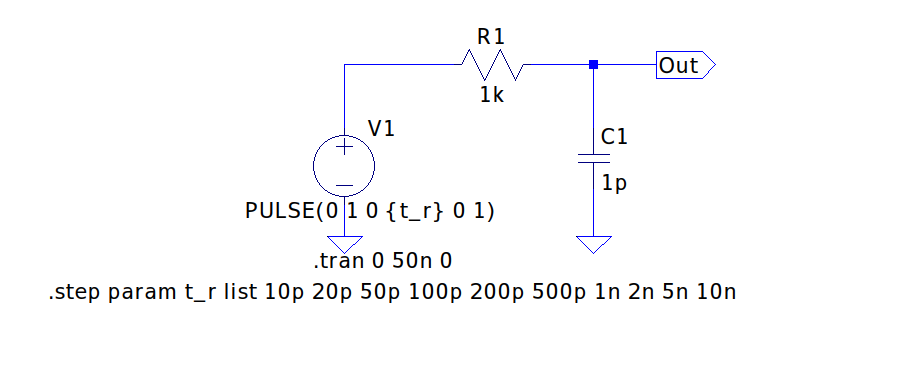
\includegraphics[scale=0.45]{./figs/Q5_tb.png}
\subsection*{(a)}
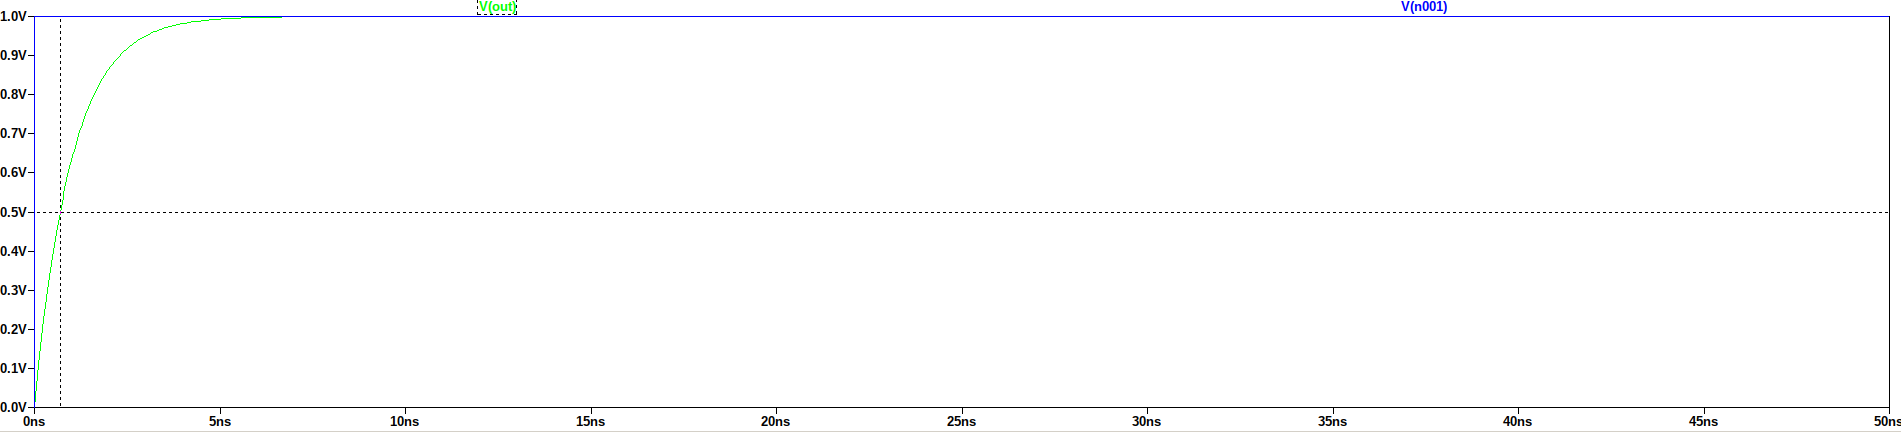
\includegraphics[scale=0.28]{./figs/Q5.png}\\
$t_{p, simulated}$ = 692ps\\
$t_{p, calculated}$ = RCln(2) = 693.14ps
\subsection*{(b)}
Now from the SPICE simulations with different rise time from 10ps to 10ns, and Propagation delay is observed and plotted using python with log-lin.\\
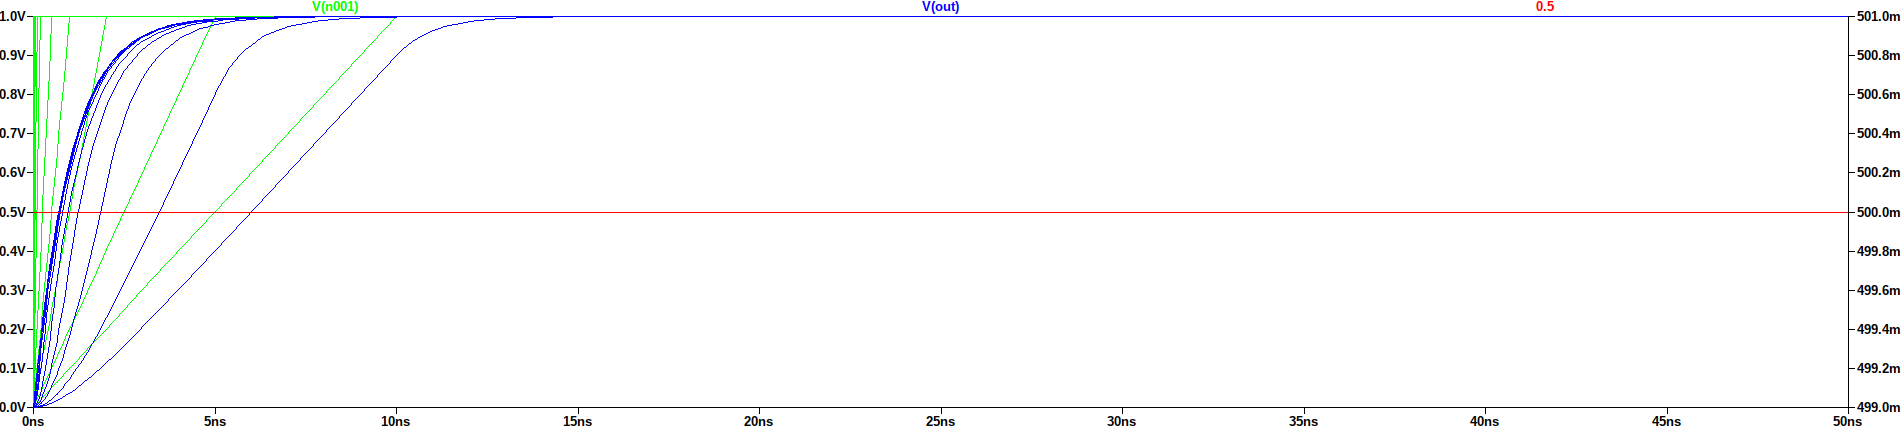
\includegraphics[scale=0.28]{./figs/Q5_b_plots.png}\\

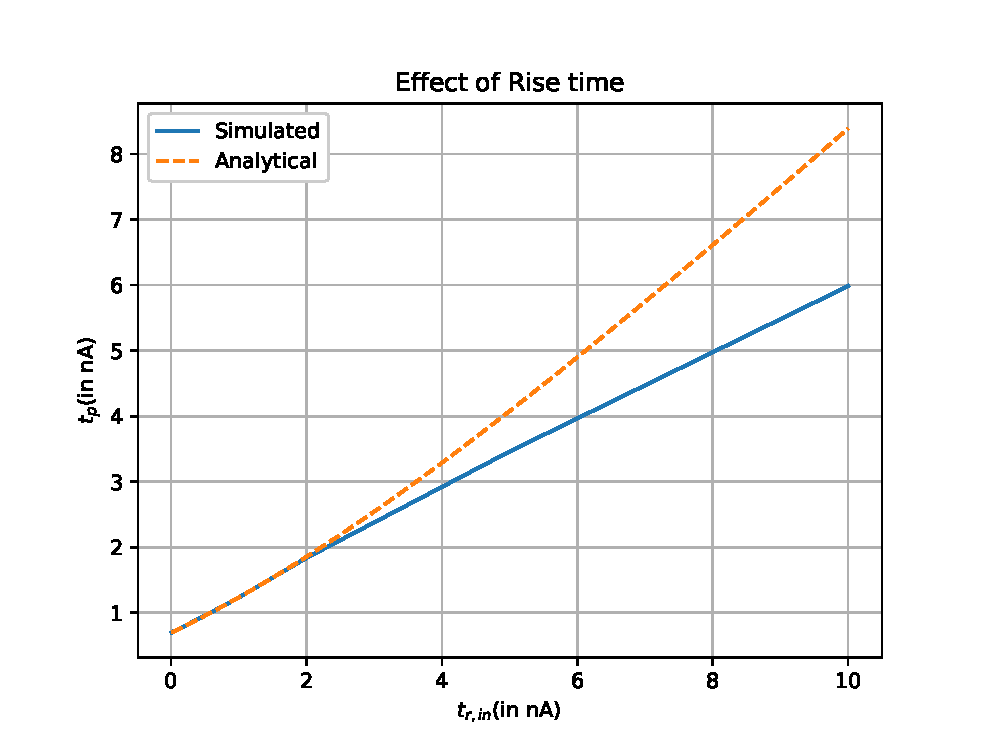
\includegraphics[scale=0.7]{./figs/Q5_b.eps}\\
The analytical expression is evaluated in (c).

\subsection*{(c)}

The input can be interpreted as differnce two ramp signals where one is delayed by $t_r$.
\begin{gather*}
V_{in}(t) = \frac{r(t) - r(t - t_r)}{t_r}\\
\implies V_{in}(s) = \frac{\frac{1}{s^2} - \frac{e^{-st_r})}{s^2}}{t_r} \implies V_{in}(s) = \frac{1}{s^2}\left(\frac{1 - e^{-st_r}}{t_r}\right)\\
V_{out}(s) = V_{in}(s) \frac{1}{1 + s\tau} \implies V_{out}(s) = \frac{1}{s^2}\left(\frac{1 - e^{-st_r}}{t_r}\right)\frac{1}{1 + s\tau}\\
V_{out}(s) = \frac{1}{t_r}\left(\left(\frac{1}{s^2(1 + s\tau)}\right) - \left(\frac{e^{-st_r}}{s^2(1 + s\tau)}\right)\right)\\
V_{out}(t) = \frac{1}{t_r}\left(\left(t - \tau + {\tau}e^{-\frac{t}{\tau}}\right) - \left(t - t_r - \tau + {\tau}e^{-\frac{t-t_r}{\tau}}\right)\right)\\
\implies \tcbhighmath[drop fuzzy shadow]{V_{out}(t) = 1 - e^{\frac{-t}{\tau}}\left(\frac{e^{\frac{t_r}{\tau}} - 1}{t_r/{\tau}}\right)}
\end{gather*}
Where $\tau$ is RC and $t_r$ is rise time.\\
According to defination of propagation delay $V_{out}(t_p)$ = 0.5V.\\
\begin{gather*}
0.5 = 1 - e^{\frac{-t_p}{\tau}} \left(\frac{e^{\frac{t_r}{\tau}} - 1}{t_r/{\tau}}\right)\\
\implies \tcbhighmath[drop fuzzy shadow]{t_p = RCln \left(2\left[\frac{e^{\frac{t_r}{RC}} - 1}{t_r/{RC}}\right]\right)}
\end{gather*} 
When $t_r -> 0$, $t_p -> RCln2$. 
\end{document}
